
% Basic setup. Most papers should leave these options alone.
\documentclass[a4paper,fleqn,usenatbib]{../mnras}

%\usepackage{newtxtext,newtxmath}

% Use vector fonts, so it zooms properly in on-screen viewing software
% Don't change these lines unless you know what you are doing
\usepackage[T1]{fontenc}
\usepackage{ae,aecompl}


%%%%% PACKAGES %%%%%

% Only include extra packages if you really need them. Common packages are:
\usepackage{graphicx}	% Including figure files
\usepackage{amsmath}	% Advanced maths commands
\usepackage{amssymb}	% Extra maths symbols
\usepackage{color}
\usepackage{enumerate}

%%%%% CUSTOM COMMANDS %%%%%

\newcommand{\Nant}{\ensuremath{N_{\mathrm{a}}}}
\newcommand{\Ng}{\ensuremath{N_{\mathrm{g}}}}
\newcommand{\s}{\ensuremath{\hat{\mathbf{s}}}} % s-hat for sine-projected direction
\newcommand{\spix}{\ensuremath{\hat{\mathbf{s}}_{0}}}
\newcommand{\Cna}[1][n]{\ensuremath{\mathcal{C}^{(#1)}_{a,\spix}}}
\newcommand{\Kna}[1][n]{\ensuremath{\mathcal{K}^{(#1)}_{a,\spix}}}
\newcommand{\ri}{\ensuremath{\mathbf{r}_i}}
\newcommand{\ra}{\ensuremath{\mathbf{r}_a}}
\newcommand{\rb}{\ensuremath{\mathbf{r}_b}}
\newcommand{\beamr}{\ensuremath{\widetilde{W}}}
\newcommand{\beamtheta}{\ensuremath{W}}
\newcommand{\Er}[1]{\ensuremath{\widetilde{E}_{#1}}}
\newcommand{\Erest}[1]{\ensuremath{\widetilde{E}'_{#1}}}
\newcommand{\Ethetaest}{\ensuremath{E'}}
\newcommand{\V}{\ensuremath{\widetilde{V}}}
\newcommand{\dif}{\mathrm{d}}
\newcommand{\caliter}{400}
\newcommand{\damp}{\ensuremath{\gamma}}
\newcommand{\itr}{20}
\newcommand{\tcal}{\ensuremath{t_{\mathrm{cal}}}}
\newcommand{\teff}{\ensuremath{t_{\mathrm{eff}}}}

%%%%%%%%%%%%%%%%%%% TITLE PAGE %%%%%%%%%%%%%%%%%%%

% Title of the paper, and the short title which is used in the headers.
% Keep the title short and informative.
\title[EPICal]{An Efficient Feedback Calibration Algorithm for Direct Imaging Radio Telescopes
%The E-field Parallel Imaging Calibration Algorithm for Next-Generation Radio Telescopes
}

% The list of authors, and the short list which is used in the headers.
% If you need two or more lines of authors, add an extra line using \newauthor
\author[Beardsley et al.]{
Adam P. Beardsley,$^{1}$\thanks{E-mail: Adam.Beardsley@asu.edu}
Nithyanandan Thyagarajan,$^{1}$
Judd D. Bowman$^{1}$
\newauthor
and Miguel F. Morales$^{2}$
\\
% List of institutions
$^{1}$Arizona State University, School of Earth and Space Exploration, Tempe, AZ 85287, USA\\
$^{2}$University of Washington, Department of Physics, Seattle, WA 98195, USA\\
}

% These dates will be filled out by the publisher
\date{Accepted XXX. Received YYY; in original form ZZZ}

% Enter the current year, for the copyright statements etc.
\pubyear{2016}

% Don't change these lines
\begin{document}
\label{firstpage}
\pagerange{\pageref{firstpage}--\pageref{lastpage}}
\maketitle

% Abstract of the paper
\begin{abstract}
We present the E-field Parallel Imaging Calibration (EPICal) algorithm, which addresses the 
need for a real-time calibration method for direct imaging radio astronomy correlators. Direct 
imaging involves a spatial fast Fourier transform of antenna \textbf{signals}, alleviating 
\textbf{an 
$\mathcal{O}(\Nant^2)$ computational bottleneck typical in radio correlators, and yielding a more gentle $\mathcal{O}(\Nant \log_2 
\Nant)$ scaling.} \textbf{This} can save orders of magnitude in computation cost for next generation arrays 
consisting of hundreds to thousands of antennas. However, because signals are mixed in the 
correlator, gain correction must be applied \textbf{prior to correlation, rather than on visibilities post-correlation.} We develop the EPICal algorithm 
to form gain solutions in real time without ever forming visibilities. This method scales as the 
number of antennas, and produces results comparable to those from visibilities. 
\textbf{We use simulations to demonstrate the EPICal technique and study the noise properties of
our gain solutions, showing they are similar to visibility based solutions in realistic 
situations.
By applying EPICal to Long Wavelength Array data we achieve a 65\% dynamic range
improvement compared to uncalibrated images, showing this algorithm is a promising
solution for next generation instruments.}
\end{abstract}

\begin{keywords}
instrumentation: interferometers -- techniques: image processing -- techniques: interferometric
\end{keywords}


%%%%%%%%%%%%%%%%% BODY OF PAPER %%%%%%%%%%%%%%%%%%

\section{Introduction}
In order to satisfy the survey speeds required for precision cosmology as well as searches for 
fast radio transients, radio astronomy is undergoing a paradigm shift toward interferometers 
consisting of hundreds to thousands of small, widefield antennas. Many arrays with this design 
are already built or under construction including the Hydrogen Epoch of Reionization 
Array\footnote{http://reionization.org} (HERA), the Murchison Widefield Array (MWA; 
\citealt{tin13,bow13}), the Donald C. Backer Precision Array for Probing the Epoch of 
Reionization (PAPER; \citealt{par10}), the LOw Frequency ARray (LOFAR; \citealt{van13}), the 
Canadian Hydrogen Intensity Mapping Experiment (CHIME,\citealt{ban14}), the Long 
Wavelength Array (LWA, \citealt{ell13}), and the low frequency Square Kilometer Array (SKA1-
Low \citealt{mel13}).

\textbf{The most common radio correlator designs of today, the FX and lag correlators \citep{rom99}},
cross-multiply the \textbf{signals} from all pairs of \textbf{antennas.
This} computation scales as the number of antennas squared, $\mathcal{O}(\Nant^2)$ 
\citep{bun04}. As the number of elements in future arrays grows, the computational cost will 
become prohibitively expensive, and exploring efficient correlator schemes is essential to 
enable next generation instruments \citep{lon00}. Meanwhile, radio transient monitoring 
requires access to high time and frequency resolution data to identify and characterize events 
such as fast radio bursts (FRBs, \citealt{lor07}), or to follow up gravitational wave candidates 
with radio observations \citep{abb16a,abb16b}. FRBs are highly unexplored at low frequencies 
(< 1 GHz), but are expected to occur on timescales $\Delta t \sim$ 1--10~ms \citep{tho13}. 
Recording the full visibility matrix for $\Nant \gtrsim 10^3$ arrays at this timescale leads to 
extremely high data write rates. 

Direct imaging correlators are a new variety of radio correlator which aim to alleviate both the 
computational strain of forming $\Nant^2$ correlations and the high data throughput associated 
with short timescale science. This is done by performing a spatial fast Fourier transform (FFT) 
to image the antenna signals, then squaring and averaging in time. This process scales as 
$\mathcal{O}(\Ng \log_2 \Ng)$, where \Ng~is the number of grid points in the FFT \citep{mor11,
 teg09, teg10}. For certain classes of telescopes, significantly those envisioned for next 
 generation cosmology experiments, this scaling is a large improvement over the $\Nant^2$ 
 scaling of traditional methods. Furthermore, because images are generated \textbf{in real-time}, the native 
 output bandwidth will be lowered \textbf{in cases where $\Ng < \Nant^2$}, and has the potential to be 
 lowered even further with \textbf{real-time} transient processing.

A handful of prototype direct imaging correlators have been tested on arrays including the 
Basic Element for SKA Training II (BEST-2) array \citep{fos14}, the Omniscope \citep{zhe14}, 
and an earlier pulsar timing experiment at GHz frequencies \citep{oto94, dai00}. Each of these 
are examples of so-called FFT correlators -- a subclass of direct imaging correlators which rely 
on identical antennas with restricted placement, which allows the FFT to be performed without 
gridding. We recently released the E-field Parallel Imaging Correlator \citep[EPIC;][]{thy15c}, 
which is a software implementation of the Modular Optimal Frequency Fourier \citep[MOFF;][]
{mor11} imaging algorithm. This architecture leverages the software holography/A-transpose 
framework to grid electric field data streams before performing the spatial FFT, allowing for an 
optimal map without placing constraints on array layout or requiring identical antennas 
\citep{mor09,bha08,teg97a}.

A challenge common to all direct imaging algorithms is calibration of the antenna gains. With a 
traditional \textbf{cross correlator}, visibilities are written to disk and used to calibrate 
\textbf{after observing and before further processing} such as imaging. However, a direct imaging correlator mixes 
the signals from all antennas before averaging and writing to disk, making calibration a 
requirement at the front end, before imaging and averaging. Previous solutions have involved 
applying calibration solutions generated from a parallel FX correlator \citep{zhe14, fos14}, or 
integrating a dedicated FX correlator which periodically formed the full visibility matrix to solve 
for gains \citep{wij09,dev09}. While these solutions were sufficient to enable the exploration of 
FFT correlators and beamformers, they will not scale to future arrays with $\Nant \gtrsim 10^3$.

Here we present the E-field Parallel Imaging Calibration (EPICal) algorithm -- a novel solution 
to the calibration problem, which can be integrated into direct imaging correlators and scales 
only as the number of antennas, $\mathcal{O}(\Nant)$. This method uses a correlation of the 
uncalibrated antenna signal stream with an output image pixel from the backend of the 
correlator to solve for the complex gains of the antennas. Because the calibration must be 
applied before gridding and imaging, our solution requires an iterative approach where the data 
from one time series is used to update the gains which are applied to the following time series. 
An example implementation of the algorithm is available with the EPIC software 
package\footnote{http://github.com/nithyanandan/EPIC}.

We review the MOFF algorithm and derive the calibration algorithm in \S \ref{sec:math}. We 
then demonstrate the algorithm in simulations in \S \ref{sec:sim}, 
\textbf{and discuss noise trends in \S \ref{sec:noise}. We then apply the algorithm to a sample LWA 
data set in \S \ref{sec:data}}.
Finally we conclude and discuss potential extensions to the 
algorithm in \S \ref{sec:discussion}.

\section{Mathematical Framework}\label{sec:math}
\subsection{Review of the MOFF algorithm}
We begin by reviewing the data flow of the MOFF algorithm, highlighting aspects relevant to 
the calibration. The interested reader is encouraged to refer to \citealt{mor11} for a more 
thorough discussion. Figure~\ref{fig:moff_flow} is reproduced from \citealt{thy15c} to illustrate 
the various steps of the algorithm.

\begin{figure}
\begin{center}
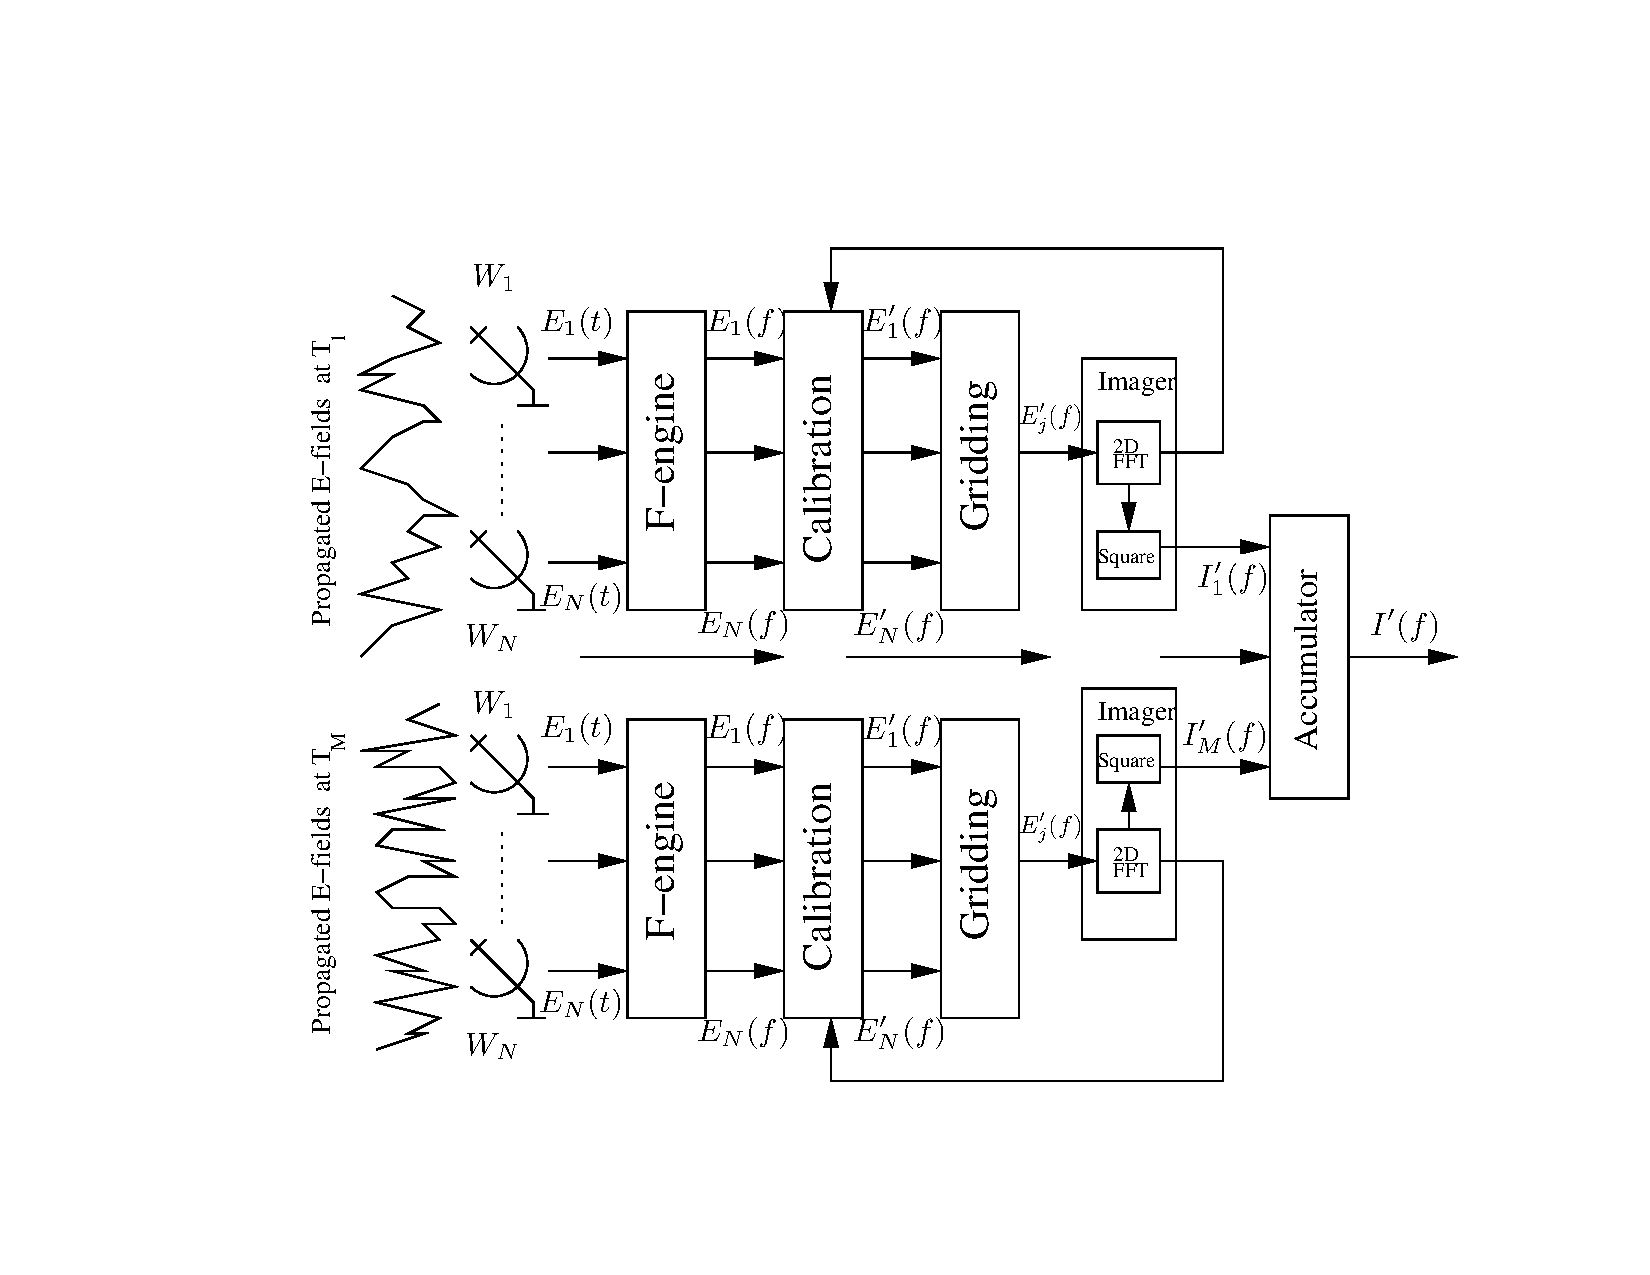
\includegraphics[width=\columnwidth]{fig1.pdf}
\caption{Data flow for the MOFF algorithm, reproduced from \citealt{thy15c}. The time ordered 
electric field \textbf{measurements} are collected by the antenna elements then frequency transformed in the 
F-engine. The calibration is applied, then the electric field measurements are gridded using the 
\textbf{antenna aperture illumination patterns}. The imager performs a spatial 2D FFT on the gridded data before 
squaring and averaging. The accumulated images are then written to disk.}
\label{fig:moff_flow}
\end{center}
\end{figure}

%%% New text
\textbf{We begin by considering the electric field vector incident on the ground as a function of time, 
$\mathbf{E}(\mathbf{r},t)$. The position vector, $\mathbf{r}$, is measured from some arbitrary 
origin. Following \citealt{cla99} we make a few assumptions in order to clarify notation and 
simplify the problem. First we note that the time ordered electric field can be expressed as a 
Fourier series with coefficients corresponding to frequencies $f$. This allows us to analyze the 
quasi-monochromatic components of the electric field, $\mathbf{E}(\mathbf{r},f,t)$, with the 
understanding that the full field is composed of all components and their corresponding Fourier 
functions. We retain the time dependence because in practice each Fourier component will only be 
measured over discrete sampling intervals. }

\textbf{It is convenient to simplify notation by expressing the position vector in units of wavelengths relative to the monochromatic component of interest, 
$\mathbf{r}\rightarrow \mathbf{r}/\lambda$. We will also assume all antennas lie in a plane, 
reducing the problem to two dimensions. While the MOFF algorithm in principle can account for 
non-coplanar arrays through the W-projection algorithm \citep{cor08}, the EPIC code does not 
currently support this so we leave it to future work.}

\textbf{Next we treat the electric field as a scalar quantity, ignoring polarization effects. This allows us 
to express the electric field as a scalar, $E(\mathbf{r},f,t)$, and treat subsequent field 
propagation and measurements as scalar rather than tensor multiplications. A full polarization 
treatment is required to construct polarized sky images, however the calibration will only 
require a sky model expressed in the instrumental polarization basis. We can therefore treat 
each instrument polarization independently.}

\textbf{Finally we assume the sources of the electric field are far away, allowing us to describe the 
electric fields propagating from sky sources as originating from an imaginary celestial sphere 
located a large distance from the ground. We express this intermediary electric field as an 
angular distribution, $\mathcal{E}(\hat{\mathbf{s}},f,t)$, where $\hat{\mathbf{s}}$ is the unit 
vector in the direction of a patch of the celestial sphere. We further assume the space between 
the celestial sphere and the ground is empty, allowing us to express the electric field incident 
on the ground as a Fourier integral of the propagated fields across the hemisphere above the horizon.
\begin{equation}\label{eq:sky_propagated}
E(\mathbf{r},f,t) = \int \mathcal{E}(\hat{\mathbf{s}},f,t) e^{-2\pi i \mathbf{r} \cdot \hat{\mathbf{s}}}\, d\Omega
\end{equation}  
By making the latter assumptions we have left treatment of the ionosphere and terrestrial 
emission such as local interference or thermal radiation from the ground for future work. }

\textbf{Next we turn to the measurement performed by an antenna with far-field radiation pattern 
$\mathcal{W}_a(\hat{\mathbf{s}})$, where the subscript $a$ denotes a specific antenna. We 
adopt the common convention of normalizing the radiation pattern to have response of unity at the 
center of the main lobe \citep[e.g.][]{nap99}. Consequently, the translation between the terminal 
voltages to electric field measurements has been absorbed in our definition of the radiation 
pattern. The ideal antenna electric field measurement can be expressed as 
\begin{equation}
E^I_a(f,t) = \int \mathcal{W}_a(\hat{\mathbf{s}})\mathcal{E}(\hat{\mathbf{s}},f,t) e^{-2\pi i \mathbf{r} \cdot \hat{\mathbf{s}}}\, d\Omega. 
\end{equation}
Equivalently we can express the effect of the antenna radiation pattern in the plane of the 
aperture.
\begin{equation}
E^I_a(f,t) = \int_{\mathrm{aperture}}W_a(\mathbf{r}-\mathbf{r}_a)E_a(\mathbf{r},f,t)\,d^2\mathbf{r}
\end{equation}
Here we used the Fourier relationship between the antenna's far-field radiation pattern and the 
aperture illumination pattern (sometimes referred to as the aperture distribution), 
\begin{equation}
W_a(\mathbf{r}-\mathbf{r}_a)=\int  \mathcal{W}_a(\hat{\mathbf{s}}) e^{-2\pi i \mathbf{r} \cdot \hat{\mathbf{s}}}\, d
\Omega.
\end{equation} 
While it is possible to define each antenna aperture illumination pattern in a way to absorb the 
relative position of the antenna, we keep the $\mathbf{r}_a$ coordinate to retain the separable
concepts of the primary beam (the product of two antenna radiation patterns) and the array
point spread function (square of the Fourier transform of the array layout).}

\textbf{The first step of the MOFF algorithm is to digitize the antenna signals and perform an FFT to 
channelize the time-ordered data. This is effectively estimating the quasi-monochromatic 
components of the electric field. The sampling rate of the digitization 
determines the bandwidth of the observation, and the sampling period determines the minimum 
frequency channel resolution. The frequency Fourier transform operation is often referred to as 
the F-engine of a correlator. The MOFF shares the same F-engine design as an FX cross
correlator which performs the frequency transform (F-engine) before cross multiplying 
(X-engine). }

Thus far we have \textbf{considered the perfectly measured electric field distribution according to 
the antenna far-field radiation patterns}. Here we introduce a multiplicative complex gain as 
well as an additive noise term which corrupt the measured signals.
\begin{equation}\label{eq:apply_gain}
E_a(f,t) = g_a(f,t) E_a^I(f,t) + n_a(f,t)
\end{equation}
\textbf{We have carried the frequency dependence to this point to make clear the complex gains are
frequency dependent. However,} each subsequent step treats each frequency 
channel independently, so we will drop the $f$ to simplify notation. 
\textbf{Furthermore, while antenna gains may vary with time, we will assume they are constant over
the period of our calibration, and thus drop their time dependence from the notation.}

The MOFF algorithm next calls for a calibration \textbf{of the electric field measurements}. The goal of our new calibration method will be 
to form an estimate of the gains, $g'_a$, \textbf{where the prime represents an estimate}. For now we will assume we have formed an estimate 
to proceed with the MOFF pipeline. We correct the incoming electric field data stream using our 
current estimate of the gains.
\begin{equation}
E'_a(t) = E_a(t)/ g'_a
\end{equation}

The next step is to grid the \textbf{calibrated electric field measurements to a finite set of regularly spaced 
positions on the plane of the ground, $\mathbf{r}_j$.
The extent of the grid is chosen to encompass the footprint of the antenna array.
MOFF uses the antenna aperture illumination patterns as the} gridding 
kernel according to the software holography/A-transpose technique \citep{mor09,bha08}. 
\textbf{Mathematically we can express the gridding operation as}
\begin{equation}\label{eq:gridding}
E'_j=\sum_a W_a(\mathbf{r}_j-\mathbf{r}_a) E'_a(t)
\end{equation}
\textbf{Formally each pixel is calculated by summing over all antennas and their aperture illumination patterns.
However the aperture illumination patterns are typically compact and non-overlapping, so most pixels
will only contain contribution from one antenna, allowing equation~\ref{eq:gridding}
to be calculated through a sparse matrix multiplication.}
This gridding 
achieves an optimal map \citep{teg97b} and places the data on a regular grid. Unlike 
traditional correlators which grid visibilities, the MOFF grids the electric field measurements directly. This 
operation must be performed for every time sample, before any averaging of the data.

After gridding, the imaging portion of the MOFF performs a 2D spatial FFT to form 
instantaneous electric field images of the sky \textbf{at fixed locations $\s_k$.
The Fourier dual coordinates to $\mathbf{r}$ are $(l,m)$, where $l=\sin\theta\cos\phi$,
$m=\nobreak\sin\theta\sin\phi$, and $(\theta,\phi)$ are the zenith 
and azimuthal angles. The full unit vector towards the sky is 
$\s=(l,m,\sqrt{1-l^2-m^2})$.
The sample spacing and resolution of $\s_k$ are given 
by the choices of $\mathbf{r}_j$ grid parameters, according to the usual FFT relations. 
Fine $\mathbf{r}_j$ grid spacing can result in non-physical angular pixels ($l^2+m^2>1$),
which should be discarded.}

The pipeline up to this point can be summarized 
through the following equation.
\begin{align}
\mathcal{E}'(\s_k,t) & = \underbrace{\frac{1}{\Nant} \sum_j e^{2\pi i \mathbf{r}_j \cdot \s_k}}_{\mathrm{2D\;FFT}} 
\underbrace{\sum_a W_a(\mathbf{r}_j - \ra)}_{\mathrm{Gridding}} \\
& \qquad \times \underbrace{ \frac{1}{g'_a} \left(g_a E_a^I(t)+n_a(t)\right)}_{\mathrm{Calibration}} \nonumber
\end{align}
The sum over antennas uses the \textbf{antenna aperture illumination pattern} to grid the calibrated electric field \textbf{measurements} onto 
regular gridpoints, $\mathbf{r}_j$. The \textbf{sum over $j$} denotes the 2D FFT to sky coordinates, resulting in an 
estimate for the instantaneous electric field image. We can simplify this expression by 
exchanging the sums \textbf{and use the DFT to approximate the Fourier relationship between
the antenna aperture illumination pattern and the far-field radiation pattern.}
\begin{align}\label{eq:epix}
\mathcal{E}'(\s_k,t) & = \frac{1}{\Nant} \sum_a \frac{1}{g'_a}\left(g_a E^I_a(t)+n_a(t)\right) e^{2\pi i \s_k \cdot \ra} \nonumber \\
  & \qquad\times \sum_j W_a(\mathbf{r}_j-\ra)e^{2\pi i \s_k \cdot (\mathbf{r}_j-\ra)} \nonumber\\
& \approx \frac{1}{\Nant} \sum_a \frac{1}{g'_a}\left(g_aE^I_a(t)+n_a(t)\right) e^{2\pi i \s_k \cdot \ra}\mathcal{W}_a(\s_k)
\end{align}
In this form we see that the effect of gridding with the antenna \textbf{aperture illumination pattern} is to attenuate 
the image by a factor of the \textbf{far-field radiation response, $\mathcal{W}_a(\s)$.}

Finally, the images are squared and averaged in time to form \textbf{dirty images, 
$I'(\hat{\mathbf{s}}_k)$, then} written 
to disk. While operations have been reordered, the resulting image is equivalent to one 
produced by gridding and imaging visibilities. By shifting from cross-correlation of all pairs of 
antennas to a spatial FFT, the computational cost is significantly lowered for certain classes of 
compact arrays. The output bandwidth is also greatly reduced \textbf{in many scenarios} as visibilities are exchanged for 
gridded images. A full exploration of these scalings was presented in \citealt{thy15c}.

\subsection{Derivation of calibration}
We saw above that the MOFF algorithm (in general any direct imaging architecture) mixes the 
signal from all antennas coherently, and thus requires the calibration to be applied in real time 
at the front end of the correlator. Furthermore, visibilities are never formed, which are 
traditionally the basic measurement used to form calibration solutions. Here we derive an 
alternative method to estimate the antenna gains in real time, using the data products of the 
MOFF. 

Because the gains must be estimated in real time, we will need to use a finite stream of data to 
form an estimate which will be applied to the subsequent stream of data. Therefore the 
process of finding a solution is an iterative one. We will use parenthetical superscripts to 
denote the calibration loop number. For example, we will assume we have already formed an 
estimate from $n$ loops, $g^{(n)}_a$. We will use these estimates to calibrate the next stream 
of data in order to form an updated estimate, $g^{(n+1)}_a$.

As a starting point, we consider the feedback calibration outlined in \citealt{mor11}. There it 
was suggested to form a correlation of the uncalibrated antenna measurements with the \textbf{complex conjugate of} an image 
pixel from the output of the correlator. This is a statistically stationary quantity, which can be 
related to the sum of visibilities involving the antenna used in the correlation -- exactly the sum 
needed to calibrate \textbf{in the case of a single point source sky}. However, we aim for a more 
generalized solution for arbitrarily complex sky models. We therefore study the full expression 
for the antenna-pixel correlation,
\begin{equation}\label{eq:Kna_def}
\Kna \equiv \left<E_a^{(n)}(t) \mathcal{E}'^{*(n)}(\spix,t)\right>_t,
\end{equation}
where the superscript $n$ again represents the quantity formed in the $n^\mathrm{th}$ 
calibration loop, 
\textbf{the superscript $^*$ indicates complex conjugation,}
and \spix\, is the pixel center nearest a bright calibrator of interest. The 
following will hold for any chosen pixel, \spix, though it is advantageous to choose a pixel which 
contains a bright source to achieve a high signal to noise \textbf{ratio}. 

Plugging equation \ref{eq:epix} into equation \ref{eq:Kna_def}, 
\textbf{and substituting the $g^{(n)}_b$ for $g'_b$ to indicate the specific loop number,}
we find,
\begin{align}
\Kna & = \left<\left(g_a E_a^I(t)+n_a(t)\right) \frac{1}{\Nant} \right. \nonumber \\
& \qquad \left. \times \sum_b \frac{1}{g^{*(n)}_b}\left(g^*_bE_b^{I*}(t)+n^*_b(t)\right) e^{-2\pi i \spix \cdot \rb} \mathcal{W}^*_b(\spix)\right>_t \nonumber \\
& = \frac{1}{\Nant} \sum_b \frac{1}{g^{*(n)}_b} \mathcal{W}^*_b(\spix) e^{-2\pi i \spix \cdot \rb} \nonumber \\
& \qquad \times \left<\left(g_aE_a^I(t)+n_a(t)\right)\left(g^*_bE_b^{I*}+n^*_b(t)\right) \right>_t \nonumber \\
& = \frac{1}{\Nant} \sum_b \frac{1}{g^{*(n)}_b} \mathcal{W}^*_b(\spix) e^{-2\pi i \spix \cdot \rb} \nonumber \\
& \qquad \times \left(g_a g^*_b \left<E^I_a(t)E^{*I}_b(t)\right>_t + g_a\left<E_a^I(t)n^*_b(t)\right>_t \right. \nonumber \\
& \qquad \left. + g^*_b\left<n_a(t)E^{I*}_b(t)\right>_t + \left<n_a(t) n^*_b(t)\right>_t\right)  
%& = \frac{1}{\Nant} \sum_b \frac{1}{g^{*(n)}_b} \mathcal{W}^*_b(\spix) e^{-2\pi i \spix \cdot \rb} \left(g_ag^*_bV^I_{ab}+n_{ab}\right)
\end{align}
where in the second step we group time-dependent terms, 
and in the third \textbf{step we expanded the product within the time average.
Because the noise does not correlate with the ideal antenna measurements we can
drop the middle terms. We will also assume that the cross-correlation noise ($a\ne b$) 
is zero mean. Then by defining an ideal visibility as
$V_{ab}^I \equiv \left<E^I_a(t)E^{*I}_b(t)\right>_t$, we can simplify to}
\begin{align}\label{eq:Kna}
\Kna & = \frac{1}{\Nant} \sum_b \frac{1}{g^{*(n)}_b} \mathcal{W}^*_b(\spix) e^{-2\pi i \spix \cdot \rb}\nonumber \\
& \qquad \times \left( g_ag_b^* V_{ab}^I + \delta_{ab}\left<|n_a(t)|^2\right>_t\right)
\end{align}
\textbf{where $\delta_{ab}$ is the Kronecker-delta function. To be clear, visibilities are never directly 
formed from the data. Rather it is convenient to express $\Kna$ in terms of the ideal 
visibilities, which we can model when solving for the gains below.}

\textbf{We will ultimately wish to model the right side of equation~\ref{eq:Kna} in order to solve for the
antenna gains. However, the self-correlated noise, $\left<|n_a(t)|^2\right>$, can often be 
significantly larger than the cross correlation power, and difficult to model precisely. It 
is therefore beneficial to subtract the self-correlation directly from $\Kna$. By properly
accounting for the various weighting and phasing terms, we can use self-correlations of the
uncalibrated antenna electric field measurements to remove the corresponding
terms from equation~\ref{eq:Kna}:}
\begin{align}\label{eq:Cna}
\Cna & \equiv \Kna - \frac{1}{\Nant g^{*(n)}_a}\mathcal{W}^*_a(\spix)e^{-2\pi i \spix \cdot \ra} \left<|E_a|^2\right>_t\nonumber \\
& = \frac{g_a}{\Nant} \sum_{b\ne a} \frac{g^*_b}{g^{*(n)}_b} \mathcal{W}^*_b(\spix) e^{-2\pi i \spix \cdot \rb} V^I_{ab}.
\end{align}

The next step is to use this antenna-pixel correlation to update our gain solution. We will model 
the right hand side of equation~\ref{eq:Cna} by assuming our current gain estimates are 
approximately correct, $g^{(n)}_b\approx g_b$, and replacing the \textbf{ideal} visibilities with a set of 
model visibilities, $V^M_{ab}$. These model visibilities rely on knowledge of the sky, and should 
be precomputed \textbf{before observing}. We can then solve equation~\ref{eq:Cna} for $g_a$ to achieve an 
updated estimate.
\begin{equation}\label{eq:cal_solution}
g^{(n+1)}_a = \frac{\Cna \Nant }{ \sum_{b\ne a} \mathcal{W}^*_b(\spix) e^{-2\pi i \spix \cdot \rb} V^M_{ab} }
\end{equation}
This equation is our prescription for estimating the antenna gains of a direct imaging array. The 
\textbf{real-time} computation complexity scales as $\mathcal{O}(\Nant)$ as we form 
\textbf{an antenna-pixel correlation,} $\Cna$, for each 
antenna. 

We show schematically the process of calibrating a direct imaging correlator in 
Fig.~\ref{fig:schematic}. Computationally expensive steps that must be performed \textbf{in near real-time} 
are shown inside the gray box. The uncalibrated antenna signals are tapped out after the 
F-engine and correlated against the output image pixel of interest (i.e., equation~\ref{eq:Cna} is 
\textbf{computed in near real-time}). The correlated values are then \textbf{used to estimate the gains}
using equation~\ref{eq:cal_solution}, and additional fitting if desired. \textbf{This step does not have
the stringent cadence requirement of the steps in the gray box because the correlations have been 
averaged in time.}
The gains are then passed back 
to the correlator to update the calibration for subsequent integration intervals. 

\begin{figure}
\begin{center}
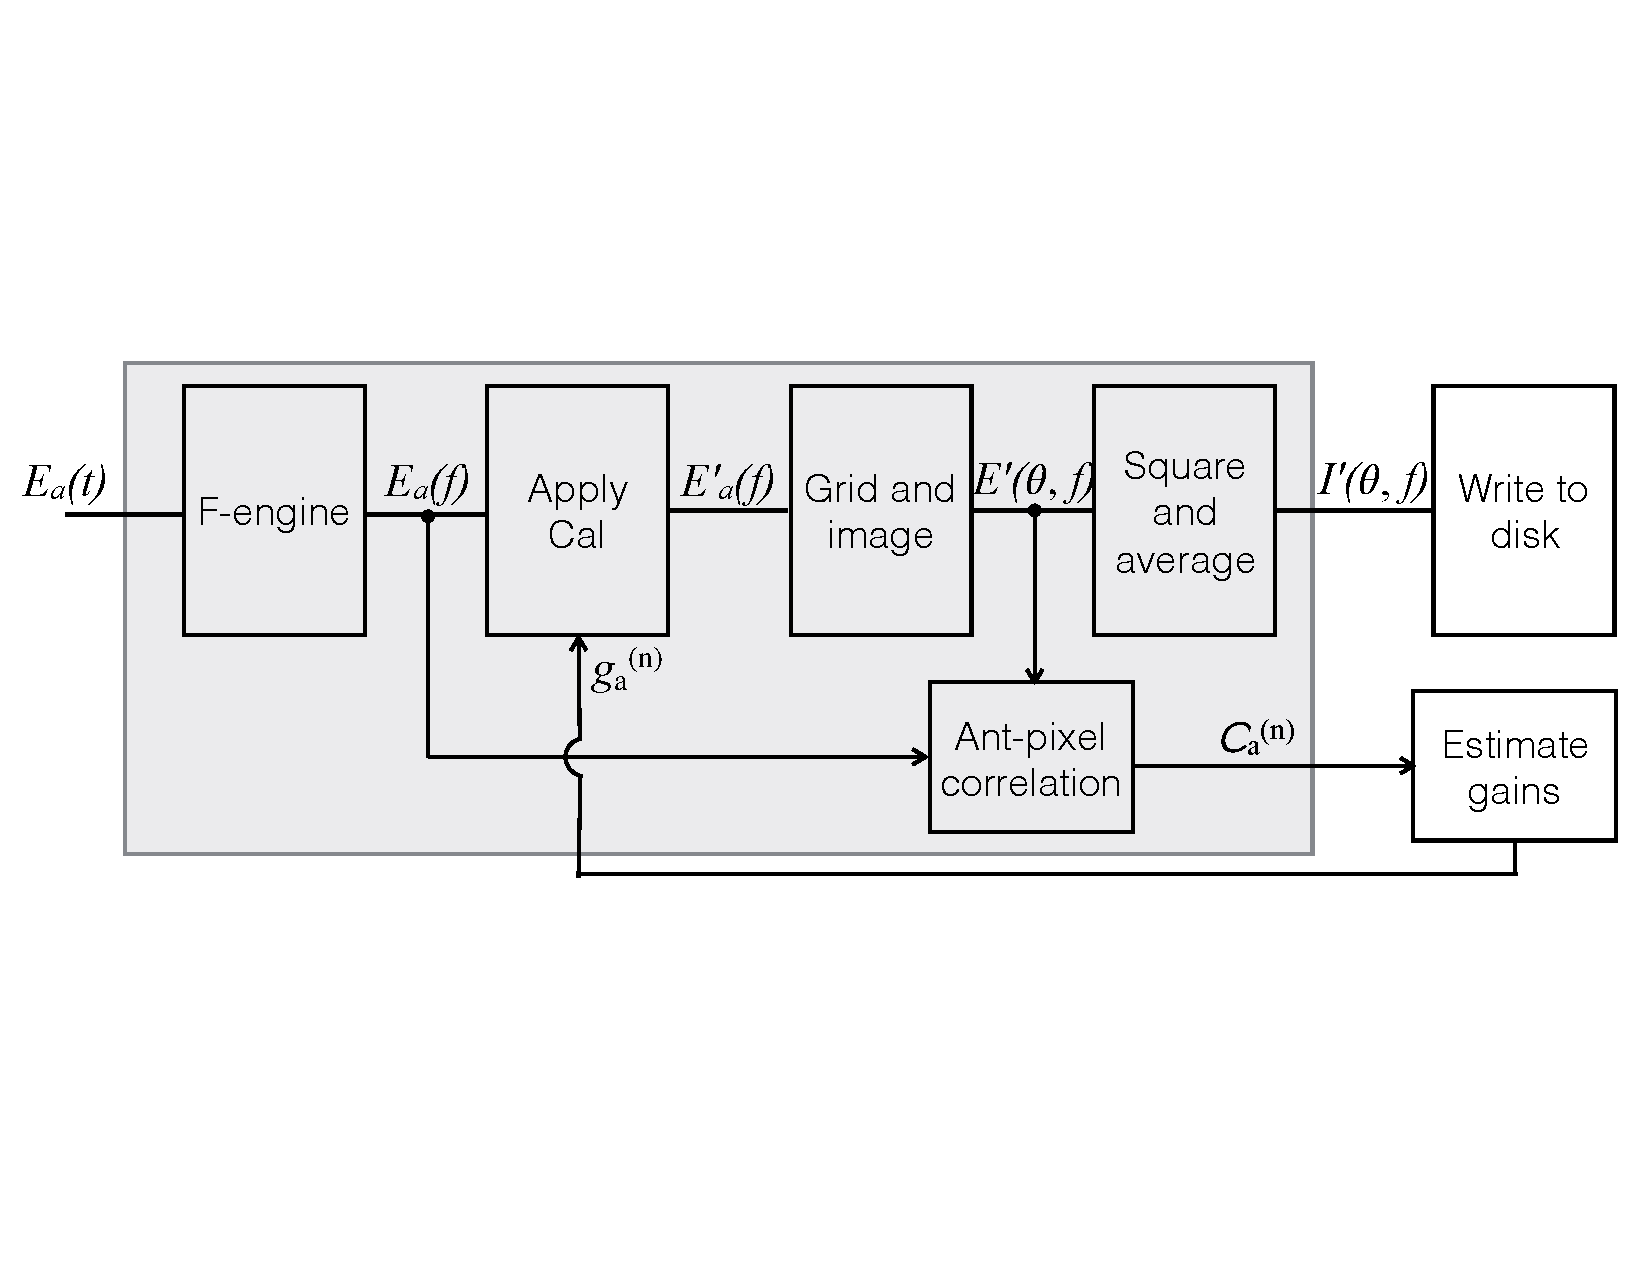
\includegraphics[width=\columnwidth]{fig2.pdf}
\caption{The general data flow of the MOFF correlator, with a feedback calibration loop. A pixel 
from the (unsquared) image is tapped out and correlated against the input antenna electric field 
\textbf{measurements} to form $\Cna$ coefficients (equation~\ref{eq:Cna}). These coefficients are then 
\textbf{used to update the gain estimates using} equations~\ref{eq:cal_solution}~and~\ref{eq:damping},
and \textbf{any additional fitting.}
The gray box shows operations which must be done at high speed (before averaging in time),
\textbf{while the} white boxes show operations which can be performed \textbf{at lower speeds because
they involve time averages quantities.}
}
\label{fig:schematic}
\end{center}
\end{figure}

While testing we found equation~\ref{eq:cal_solution} resulted in oscillatory gain solutions \textbf{over time,} 
as is often the case in iterative methods. To mitigate this we 
introduce a damping factor, $0 \leq \damp <1$, which is used to attenuate the gain update, 
effectively giving the solutions memory of previous iterations.
\begin{equation}\label{eq:damping}
%g^{(n+1)}_a = (1-\damp) g'^{(n+1)}_a + \damp g^{(n)}_a
g^{(n+1)}_a = \frac{(1-\damp)\Cna \Nant }{ \sum_{b\ne a} \mathcal{W}^*_b(\spix) e^{-2\pi i \spix \cdot \rb} V^M_{ab} }+ \damp g^{(n)}_a
\end{equation}
We found that while equation~\ref{eq:cal_solution} does indeed converge on good solutions, 
the process is made faster by tuning the damping factor. 
 Once the loop converges the damped version is 
essentially a weighted average over the past several iterations, giving it a longer effective 
integration time. 

We conclude this section by connecting our calibration expression to that found in a visibility 
framework. In the limit of a single bright calibrating source \textbf{at zenith,} we can greatly 
simplify equations~\ref{eq:Cna} and~\ref{eq:cal_solution}. We will assume the \textbf{radiation patterns} are 
normalized such that $\mathcal{W}(0)=1$. We can further drop the exponential phase terms 
because $\spix$ \textbf{is perpendicular to our planar antenna array.} We then absorb the true gains into the true visibilities in 
equation~\ref{eq:Cna} to express as a sum of measured, uncalibrated, visibilities.
\begin{equation}
\mathcal{C}^{(n)}_{a,0} \rightarrow \frac{1}{\Nant}\sum_{b\ne a} \frac{1}{g^{*(n)}_b} V_{ab}
\end{equation}

We next plug this expression into equation~\ref{eq:cal_solution} to find our simplified 
calibration solution for a single bright point source. Because our sky is a single bright point 
source, the model visibilities are simply the flux of the source, $S_{\mathrm{src}}$.
\begin{equation}
g^{(n+1)}_a \rightarrow \frac{\sum_{b\ne a}  V_{ab}/g^{*(n)}_b}{\Nant S_{\mathrm{src}}}
\end{equation}
This is simply a gain-weighted sum of the measured visibilities over the flux of the source, 
which is indeed the limiting result from a visibility approach, for example seen in \citealt{mit08}. 
The ability to recover the equivalent expression despite not actually forming the visibilities is a 
result of the fact that only sums over visibilities come into the \textbf{visibility-based} solution, as was described in 
\citealt{mor11}. We have confirmed the limiting case equivalence here, and will explore the 
more general case in more detail in \textbf{the following sections.}

\section{Simulation}\label{sec:sim}
We first demonstrate our calibration method through a controlled simulation. A complex gain is 
created for each antenna with random phase and amplitude, which is used to corrupt the 
simulated data stream, then we attempt to recover the gains using our calibration routine. The 
simulation software used is included in the EPIC package.

\textbf{Our simulated antenna 
array consists of} the inner 51 antennas of the MWA layout \citep{bea12}, within a bounding 
box of 150~m. 
\textbf{The physical parameters of our simulation can be arbitrarily scaled to other cases. However, 
we provide typical units for an MWA observation as an example. 
The antenna aperture illumination pattern} used is a 4.4~m square tophat; \textbf{a very rough 
approximation to the square shaped tiles of the MWA.} Because our algorithm treats frequency 
channels independently, we simulate only one channel. For context we treat this as \textbf{a channel
at 150~MHz with 40 kHz bandwidth, and adopt a sampling period of 25~$\mu$s. The simulated signal 
consists of 10 random point sources with flux densitities 0.5~Jy~$\lesssim S \lesssim$~1~Jy 
within the main lobe of the primary beam.}

For our unknown gains, we create a set of random complex numbers where the amplitude is 
drawn from \textbf{a gaussian distribution centered around unity with width 0.25, and truncated at zero. The gain phases are drawn from a uniform distribution between $\pm \pi$. }
These are our ``true gains", and we apply them to the frequency
domain simulated antenna electric field \textbf{measurements} as in equation~\ref{eq:apply_gain}. Our analysis is 
blind to these values until the end of the process to check accuracy. The gain estimates are 
initialized with unity, $g^{(0)}_a=1$.

We next process and image \caliter~time \textbf{samples} (10~ms). We also form the correlations, 
\Cna[0], used in our calibration loop. The pixel used for the correlation is the source with the 
largest apparent flux (intrinsic flux attenuated by the primary beam). These correlation values 
are used to update the gain estimates. \textbf{We create perfect model 
visibilities of our 10 simulated sources to be used in equation~\ref{eq:damping}. 
The updated gain estimates are} used to calibrate the following 
\caliter~time samples. Through experimentation we found a damping factor of $\damp=0.35$ 
resulted in the quickest convergence in this simulation.

The calibration loop continues by updating the gain estimates every \caliter~time \textbf{samples.} The 
phases of our gain estimates are shown in Fig.~\ref{fig:sim_phase} for 20 such iterations. 
The phase error plotted is the phase relative to the true gain for each antenna (various colored 
lines). One antenna was used as a reference to fix the absolute phase, so has zero phase 
error. The other 50 antennas are shown to have error spanning $2\pi$ initially, and after about 
10 iterations lock into a solution, settling down to noise levels around iteration \textbf{12 (0.12~s)}. We 
stop the simulation when the updated gains trace the thermal noise of the simulated sources, 
which can be seen by the coherence of the 50 antenna gains after iteration 12.

\begin{figure}
\begin{center}
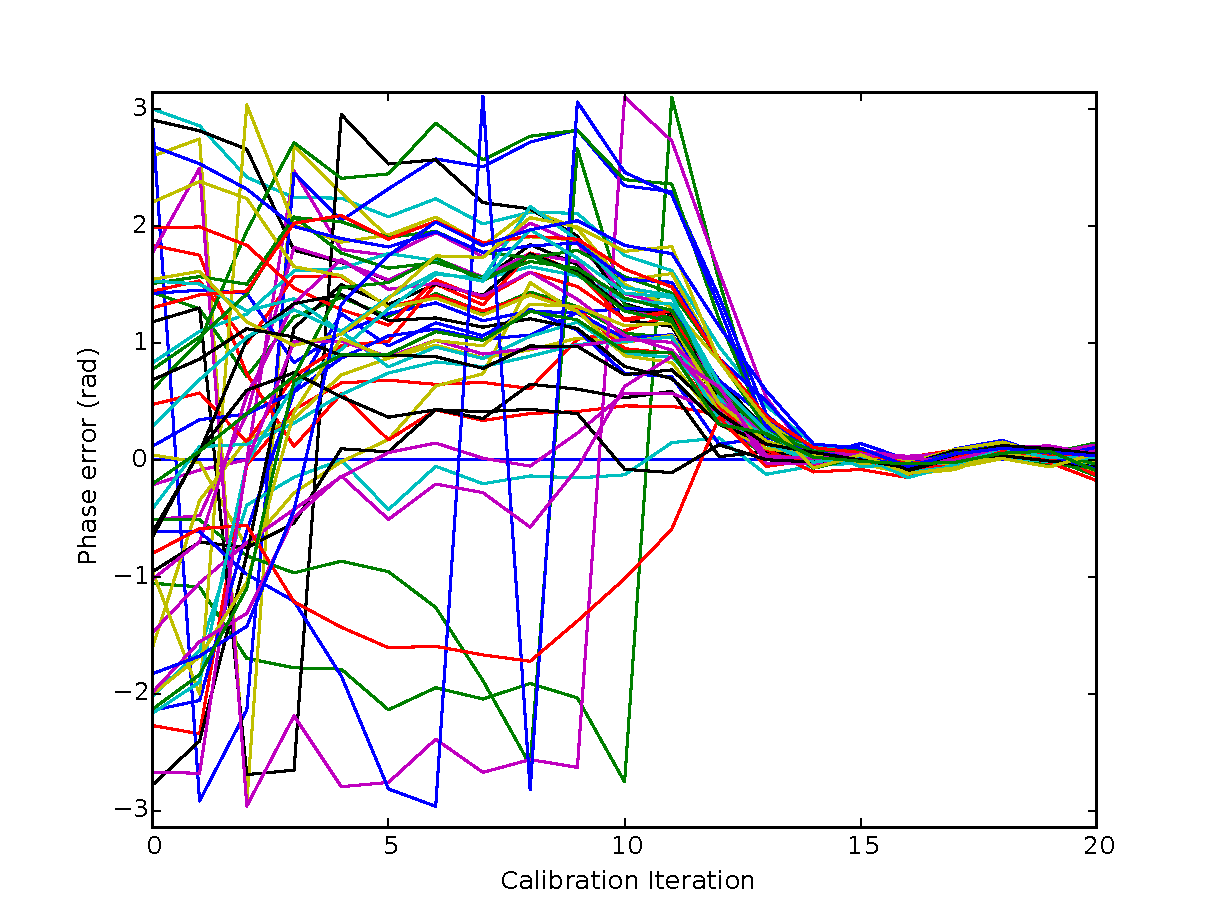
\includegraphics[width=\columnwidth]{fig3.pdf}
\caption{Phase error of gain estimates as a function of iteration for simulated calibration. The 
gains were initialized with random phases, but the calibration loop was able to recover the 
correct phases after about \textbf{12} iterations. Each line represents an antenna in our 51 MWA 
antenna sample.
}
\label{fig:sim_phase}
\end{center}
\end{figure}

The estimated gain amplitudes for the simulations are shown in Fig.~\ref{fig:sim_amp}. The 
quantity plotted is the magnitude of the estimated gains over the true gains, $\left|g^{(n)}_a/
g_a\right|$, which places all antennas on the same scale. We can see the amplitudes 
converge toward their true values around the same time as the phases (iteration \textbf{$\sim$12}). At 
the beginning of calibration we can see the \textbf{importance} of the damping factor. At $n=0$, a couple of 
gains are shown to have abnormally high amplitude estimates, notably one about 3.3 times its 
true value (red line). These unbalanced high estimates caused the entire set of gains to be 
under estimated at $n=1$, even with a damping factor of 0.35. By $n=5$ the unbalanced 
amplitudes have been damped out and the calibration continues. Without the damping factor, 
the oscillation seen in the first couple iterations would have been significantly larger and taken 
much longer to fade out. 

\begin{figure}
\begin{center}
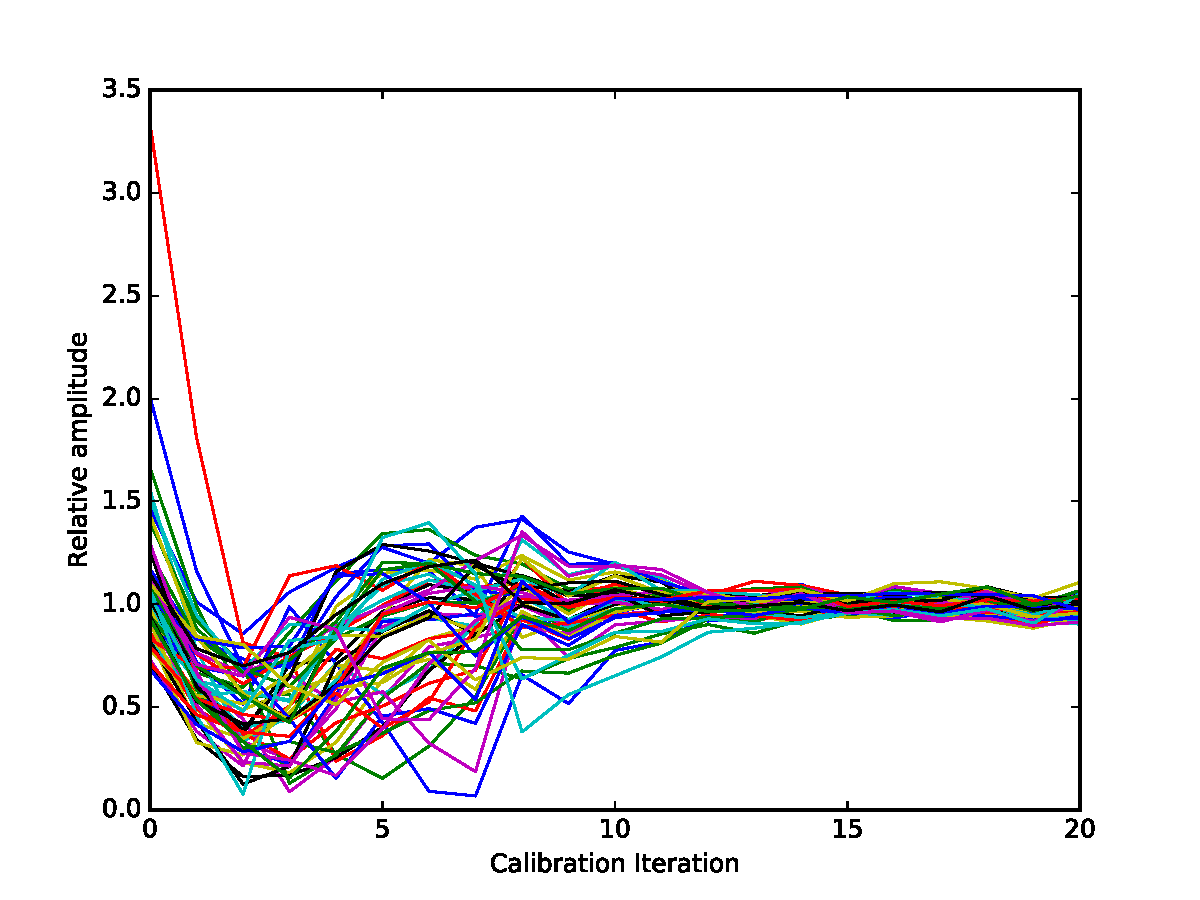
\includegraphics[width=\columnwidth]{fig4.pdf}
\caption{\textbf{Same as Fig.~\ref{fig:sim_phase}, but for gain amplitudes.
Each} line represents an antenna in the 51 MWA antenna sample. 
\textbf{The relative amplitude plotted is the magnitude of the estimated gains divided by the true gains.}
After about \textbf{12} iterations we see the 
calibration loop has settled around the correct values, with only noise remaining.}
\label{fig:sim_amp}
\end{center}
\end{figure}

After the gains have converged, we see both the phases and amplitudes continue to 
fluctuate coherently. This is due to the stochastic fluctuations of the sources 
themselves, \textbf{which are simulated as zero mean random processes with variance proportional
to their flux density.}
For this simulation we restricted each calibration 
iteration to only 10~ms integration time. In principle a calibration implementation could use 
short integration times to allow the gains to converge, then increase the integration time to 
reduce this noise.

Images created at the beginning of calibration and at the end are shown in 
Fig.~\ref{fig:sim_images}. Each image is obtained over a 400 time sample \textbf{(10 ms)} integration, corresponding to 
all snapshot images created with a given set of gain estimates. The \textbf{left} panel shows the image 
produced with our initialized unity gains. Because the phases are completely random, the 
image is essentially noise with the primary beam evident. After 20 calibration iterations, the image is far 
more clear, shown in the \textbf{middle} panel. 
\textbf{The ten sources are visible, along with rumble throughout the image. By comparing with
a perfectly calibrated image (right panel), we see that the rumble and the shapes of the
point sources are matched between the two images. We therefore conclude that the 
artifacts visible are dominated by the point spread function, rather than calibration errors.}

\begin{figure*}
\begin{center}
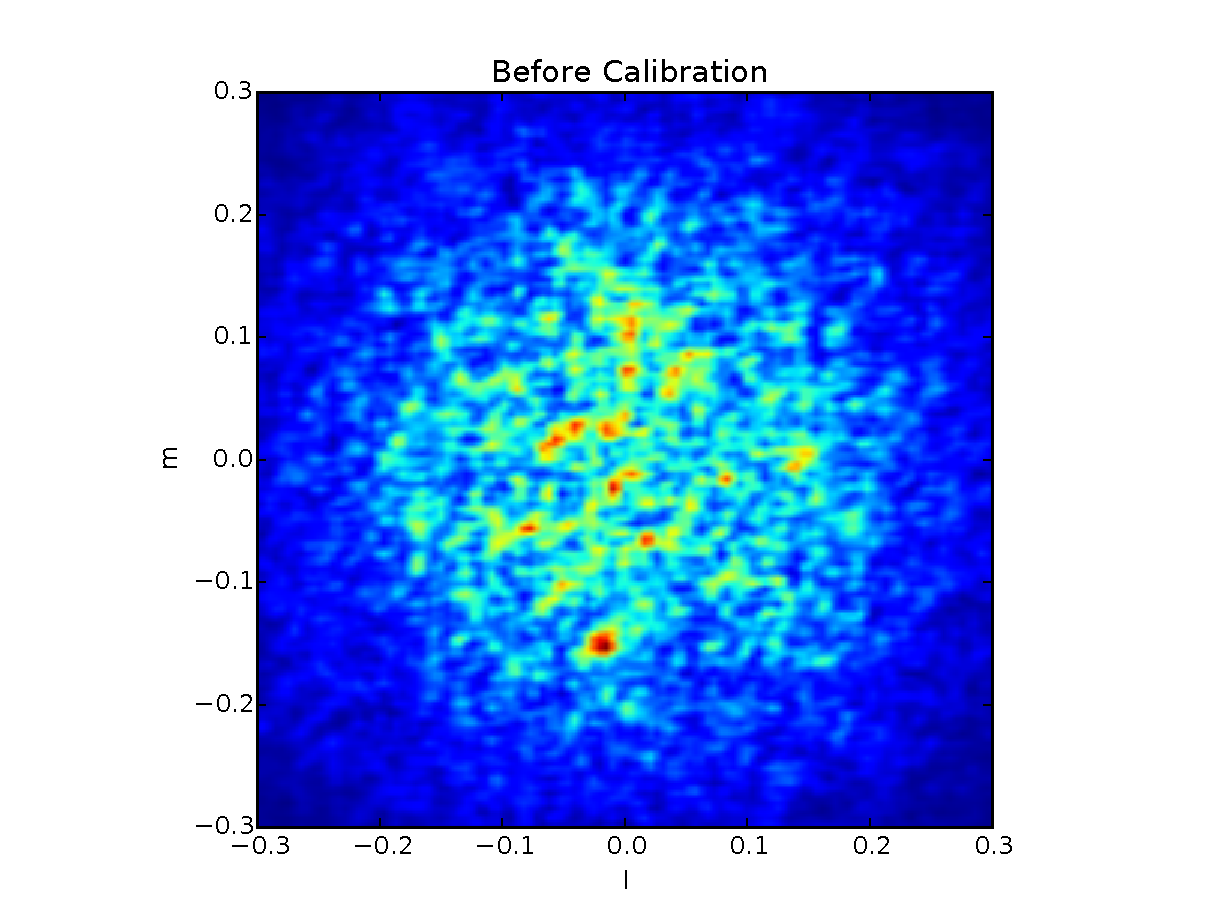
\includegraphics[width=.3\linewidth]{fig5a.pdf}
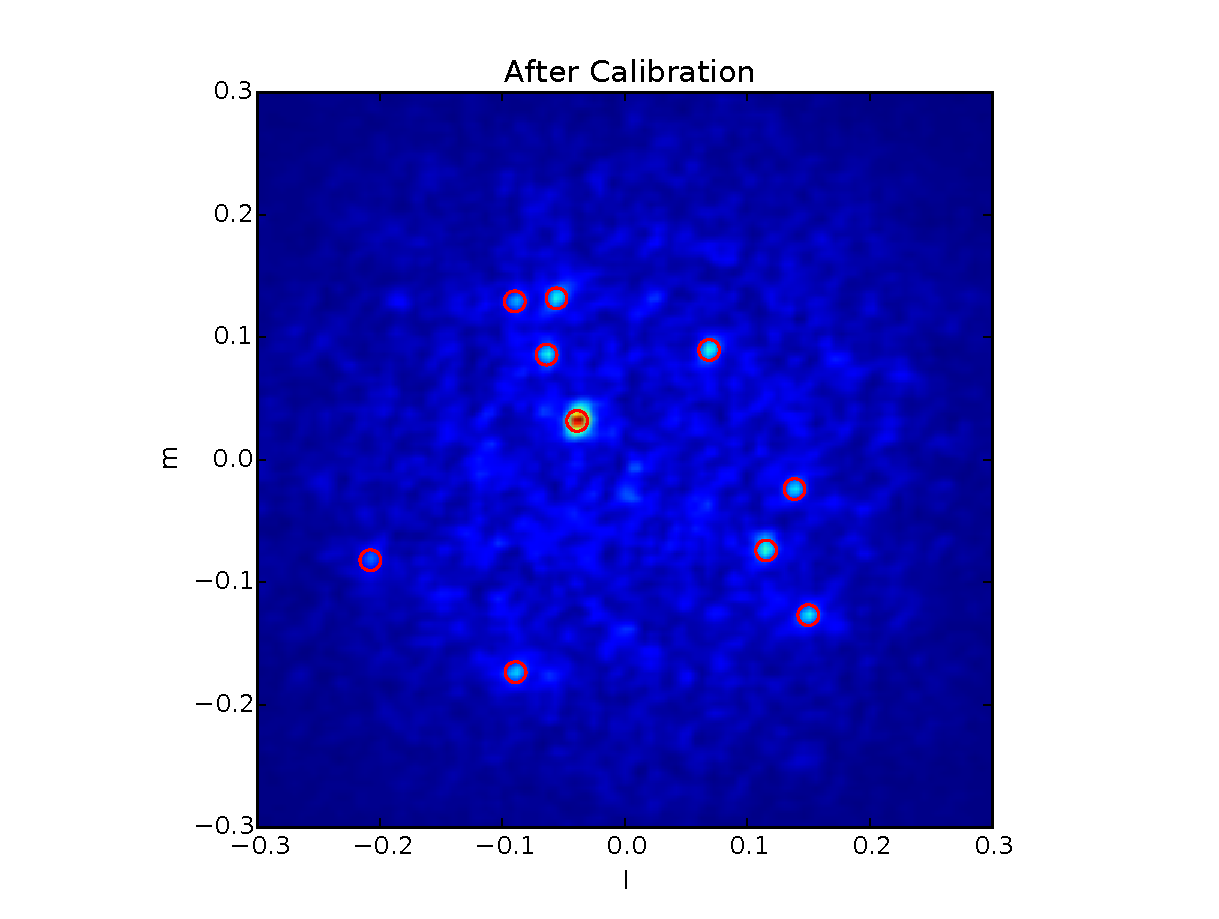
\includegraphics[width=.3\linewidth]{fig5b.pdf}
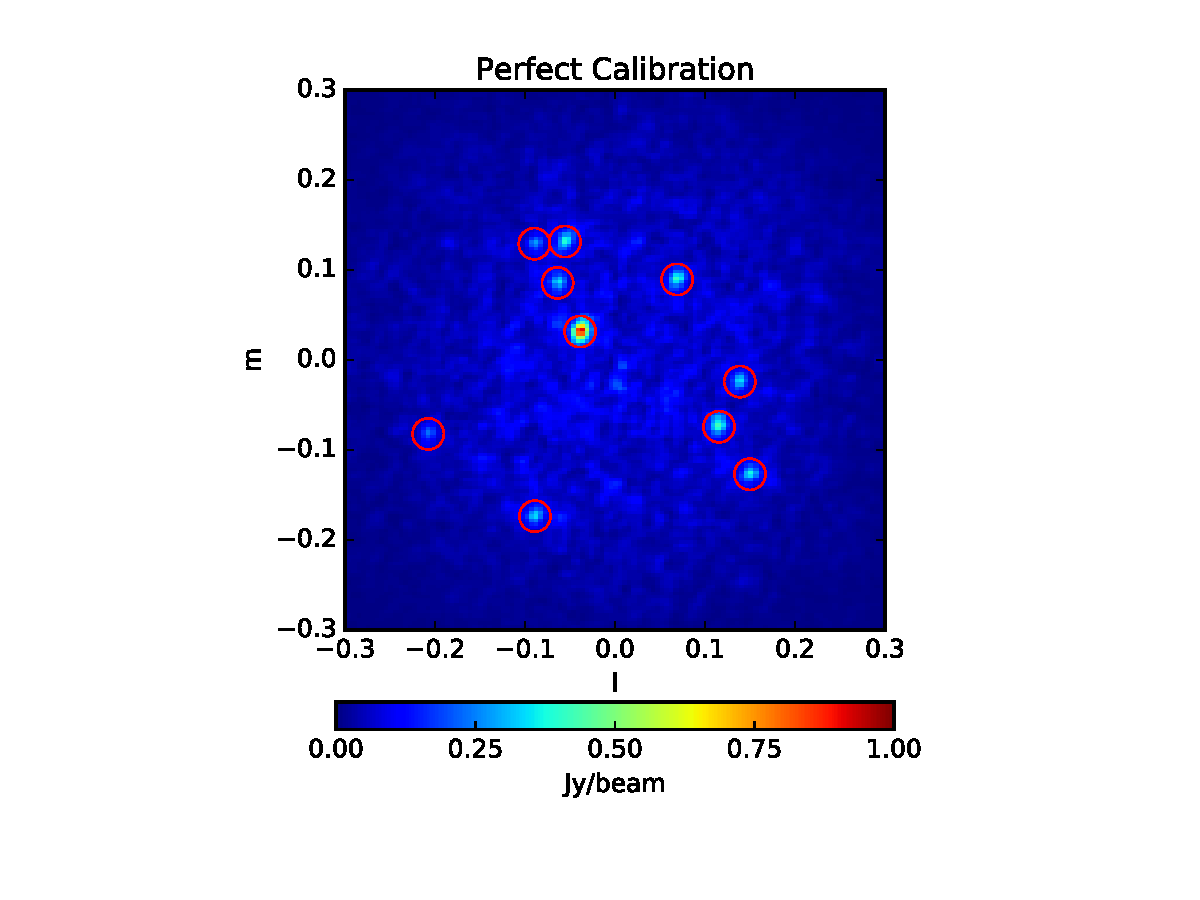
\includegraphics[width=.3\linewidth]{fig5c.pdf}
\caption{Images formed during simulated calibration. \emph{Left:} An image generated from a 
single frequency channel and \textbf{400 time sample (10 ms)} integration after the gain estimates are randomized. As 
expected with random phases, the image is completely noisy, with the shape of the primary 
beam evident. \emph{Middle:} An image formed after calibration, again with a single frequency 
channel and \textbf{400 time sample} integration. \textbf{Now the simulated point sources are visible in the image. 
\emph{Right:} An image generated from the same simulated data as the middle image, but 
with perfect calibration correction. Many of the features seen in the middle image are also
seen here, confirming that they are point spread function artifacts. The ten simulated (and modeled) point sources are highlighted with red circles.}
\label{fig:sim_images}
}
\end{center}
\end{figure*}

\section{Noise trends}\label{sec:noise}
\textbf{Next we} study the effect of noise in our system, and the consequences 
of an incomplete sky model. We run a suite of simulations varying the receiver noise and 
integration times, while forming antenna-pixel correlations, $\Cna$, for EPICal gain solutions, 
and simultaneously forming visibilities from the same \textbf{electric field measurement} streams to find visibility-based 
gain solutions for comparison. 

We use a simulated sky consisting of a 5~Jy calibrator source, and 49 other random sources 
with apparent flux densities 0.2 to 0.5 Jy (total sky power $\approx$ 23 Jy). We generated 
these sources randomly, but kept them fixed for each run. 
\textbf{We simulate the same antenna layout as in Section~\ref{sec:sim}. 
However, we increase the number of frequency channels simulated to 64, while keeping the flux of all sources constant across frequency.}
Because our calibration loop treats 
frequency channels independently, each channel can be treated as a separate trial of the 
simulation, and is used to better estimate the statistics.

To simulate receiver noise, we add a gaussian distributed complex random number to each 
antenna electric field measurement at each time \textbf{sample} according to 
equation~\ref{eq:apply_gain}. The level of the receiver noise, $\sigma_r = \left<\left|
n_a(f,t)\right|^2\right>$, is varied in different simulation runs. We include two limiting 
cases, where the receiver noise power is subdominant to the sky power ($\sigma_r = 
10.0$~Jy), and where the receiver dominates the total power ($\sigma_r=100.0$~Jy).

For each simulation run we find gain solutions using four methods:
\begin{enumerate}[i.]
\item EPICal, using a full sky model
\item EPICal, using a single point source model
\item Visibility-based, using a full sky model
\item Visibility-based, using a single point source model.
\end{enumerate}
In the cases where we use the full sky model, the model visibilities, $V^M_{ab}$, used in the 
calibration loop are created using all point sources in the simulated sky. For the single point 
source model, we only \textbf{include the bright calibrator source in the model visibilities.}
While we vary the model used for calibration, the simulated ``true sky'' remains fixed with all 50 
point sources.

For the EPICal calibration loops, we initialize our gain estimates with the true values 
(${g^{(0)}_a=g_a=1}$), and allow the estimate to be corrupted by the noise through ten 
iterations of the calibration loop. We \textbf{again} adopt a damping factor $\damp=0.35$. Because EPICal 
updates the gain estimate at each calibration loop, \tcal, but retains a memory of previous 
iterations through the damping factor, the total integration time is not straightforward. We define 
an effective integration time by considering the relative weights of each previous $\Cna$ 
contributing to the current $g^{(n)}_a$ estimate, each with integration time \tcal. In the limit $n
\rightarrow \infty$, the geometric series converges to an effective integration time of
\begin{equation}
\teff = \tcal \times \frac{1+\damp}{1-\damp}.
\end{equation}
With the damping factor we adopted here, $\teff \approx 2.1 \times \tcal$. 

We simultaneously form simulated visibilities, $V_{ab}$, by correlating all pairs of antenna \textbf{electric field 
measurements} (including the receiver noise). The \textbf{electric field measurements are correlated} for a duration equal to 
the effective integration time of the EPICal loop for comparison. We then find the 
visibility-based gain estimates by minimizing
\begin{equation}\label{eq:vis_cal}
\chi^2 = \sum_a\sum_{b\ne a} \left|V_{ab}-g_a g_b^* V^M_{ab}\right|^2,
\end{equation}
using both versions of the model visibilities described above.

 For each version of calibration, we observe the error in the gain estimates by averaging over both 
 antennas and frequency channels.
\begin{equation}\label{eq:gain_error}
\sigma_g = \left[\frac{1}{N_f \Nant} \sum_f \sum_a \frac{\left|g^{(n)}_a(f)-g_a(f)\right|^2}{\left|g_a(f)\right|^2}\right]^{1/2}
\end{equation}

The results of our simulations \textbf{for all four calibration methods are shown in Fig.~\ref{fig:errors}. }
In the case of the full sky model, we see the errors trend 
downward with longer integration times, as expected. The EPICal errors are slightly higher than 
the visibility-based errors, on average about 23\% difference. This is not surprising as EPICal 
only uses the information in a single pixel, while the visibilities use all information from the full 
sky model. However, we see that with this perfect model the errors do behave like noise
\textbf{in the sense that they integrate down with longer integrations with the expected $t^{-1/2}$ 
trend. }
\textbf{With longer integration time (or larger damping factor), EPICal can achieve the same 
level of gain error as visibility based solutions.}

\begin{figure}
\begin{center}
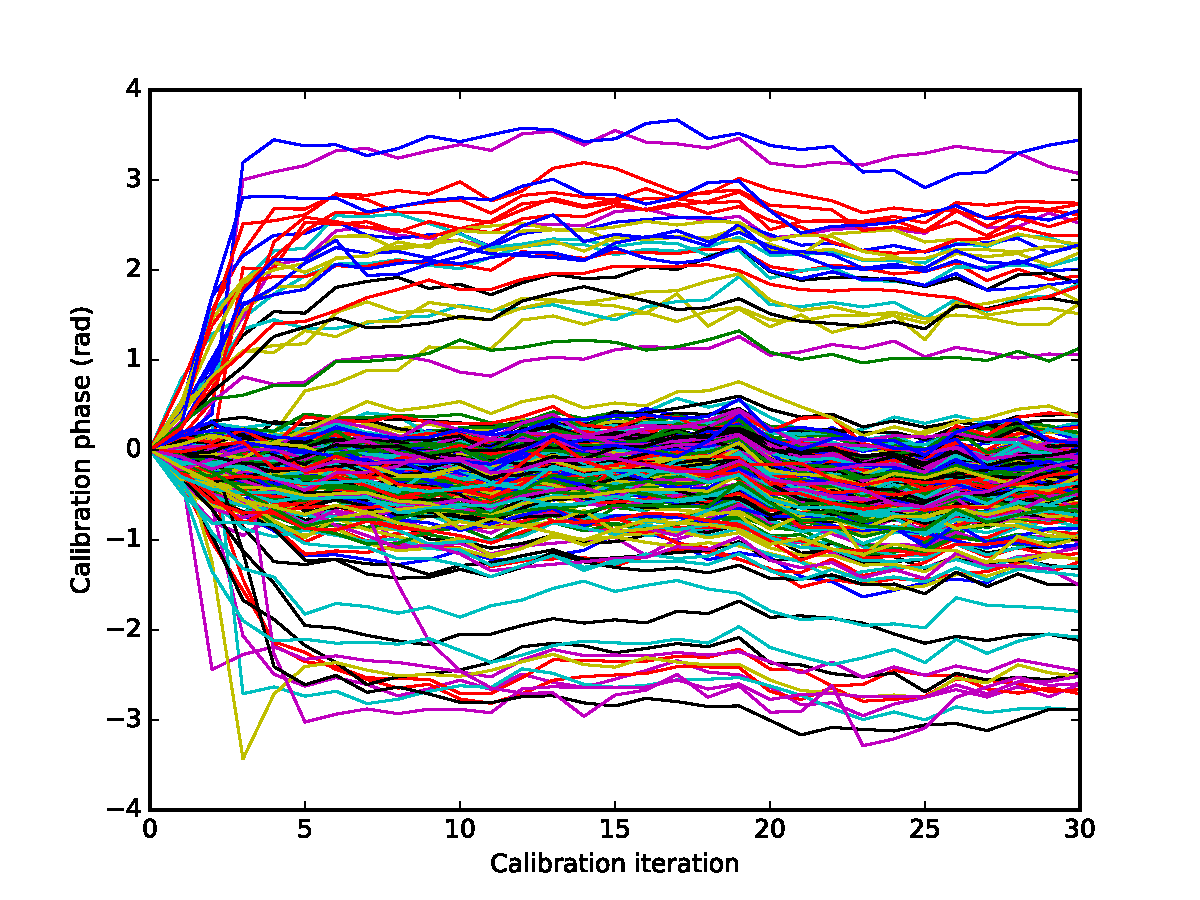
\includegraphics[width=\columnwidth]{fig6.pdf}
\caption{Gain estimate errors as a function of integration time, receiver noise (line color), and 
calibration method. The solid lines represent the error on the EPICal derived gain estimates, 
while the dashed lines represent the error on the visibility based estimates. The thicker lines 
were derived using a full sky model in the calibration loops, and the thinner lines used only a 
single point source model. In the full sky model case we see all methods trend down with 
longer integration time as expected. For a given integration time, EPICal derived errors are on 
average 23\% higher than those of visibility based calibration. In the case of a single source 
model, the errors bottom out due to the flux in the measurements that is not modeled. In this 
regime the EPICal method performs slightly better than the visibility-based method due to 
effectively beamforming to the sky pixel where the incomplete model is most accurate. On 
average EPICal errors are 5\% lower in this regime.
}
\label{fig:errors}
\end{center}
\end{figure}

The exact ratio of EPICal gain noise to visibility-based gain noise depends on the fraction of 
the total sky power contained in our calibrator source. In the example here, our calibrator 
accounted for 22\% of the total sky power. We repeated the experiment in the regime where 
the calibrator dominated the sky and found that the difference in EPICal and visibility-based 
error goes to zero, as expected. For a typical HERA observation, the sky temperature is 
expected to by about 180~K \citep{jac15}, and a bright calibrator source could be about 10\% 
of this power. In this regime we found that EPICal gain noise was about 60\% higher than 
visibility-based gain noise for the same effective integration time.

\textbf{In a more realistic situation, the observer will not have a perfectly complete model of the sky.
A common method is to instead model the brightest sources in the field,
or even a single dominant source.}
When using the single point source model, all calibration methods in Fig.~\ref{fig:errors} trend 
downward until they reach an error floor due to the confusion sources that were not modeled. 
The EPICal and visibility-based solutions reach a similar floor, but EPICal achieves a 
marginally lower level (on average 5\% lower). This can be attributed to the same reason 
EPICal underperformed with the full sky model: EPICal only used a single pixel in the sky to 
form its solutions. When using the full sky model, it was \textbf{under utilizing} the information in the 
rest of the sky. But when the sky model only contains the bright point source, the single pixel 
used in EPICal is the location where this model is most accurate, effectively down weighting 
the pixels with incomplete sky model. 
\textbf{In contrast, the visibility-based calibration method weights the apparent sky equally,
and experiences a more harsh penalty for missing sources in the model.}
In the regime typical of HERA discussed above, EPICal's 
error floor was 10\% lower than that of visibility-based solutions.

Any realistic sky model will lie somewhere between the two extremes explored here. In the 
case where the sky is modeled by a single source, as is often the case for an initial calibration, 
EPICal actually achieves smaller gain errors compared to the traditional visibility-based 
calibration. As the sky model improves, both visibility-based and EPICal gains improve, though 
the former quicker than the latter. In the limit of a perfect model, both calibration methods 
produce noise-like errors in their gains which scale down with more integration time.

\section{Application to LWA data}\label{sec:data}
We next demonstrate our calibration algorithm using an observation from the LWA station in 
New Mexico \textbf{\citep{ell13}.} The data is from the LWA narrow-band transient buffer (TBN), with time ordered 
voltage data from the 255 core antennas within a \textbf{110~m x 100~m ellipse. }
The central frequency is 74.03 
MHz, with a bandwidth of 100 kHz and \textbf{sampling period} of 5.12 ms (frequency channel 
resolution of 195.3125 Hz). For this demonstration we limit ourselves to a single polarization.

After correcting for geometric cable delays, the instrument is naturally well calibrated, as was 
seen in the demonstration of the EPIC imager in \citealt{thy15c}. However, we will aim to 
further improve on this calibration using our algorithm.

We proceed by forming model visibilities. We model only two bright objects as point sources: 
Cyg A with flux \textbf{20,539 Jy, and Cas A with flux 19,328 Jy \citep{lan12}. }
Because the raw data is attenuated by the primary beam of the instrument, we also account for 
this in our model using beam values consistent with \cite{hic12}.

We made several choices while studying the behavior of the LWA data to improve our 
calibration. Through our previous imaging work, we noted that the flux scale of uncalibrated 
images was consistent with average gain amplitudes of roughly 0.25. To allow the calibration to 
converge quickly we initialized our gain estimates at this level. 
We also found a boost in signal to noise is achieved easily by \textbf{assuming the gains are
constant across a range of frequencies, and averaging solutions across channels.}
Here we average solutions across \textbf{300} channels, or about \textbf{58.6 kHz.} 
With a fractional bandwidth $B/f_0 = 7.9 \times 10^{-4} \ll 1$, we assume a smooth bandpass 
across the band. 
A damping factor of $\gamma = 0.7$ was adopted.
\textbf{The large damping factor, relative to what was used in simulations, was necessary due to
the larger noise levels in the LWA data compared to the ideal simulations.}

Finally, we found that seven antennas\footnote{LWA antenna IDs 48, 85, 124, 148, 203, 217, 
and 244 were omitted.} produced unstable gain solutions, and in fact corrupted the entire array. 
We therefore \textbf{omitted these antennas from our analysis,} resulting in a total of 248 antennas to 
calibrate. In each calibration loop, we form $C_{i,\hat{\boldsymbol{s}}_0}, i=1,2,\ldots N_a$ and 
update our gain estimates over 10 \textbf{samples} (51.2 ms). We iterate the loop 30 times for a 
total of 1.536 seconds of data processed. The results of this calibration experiment are shown in Figs.~
\ref{fig:data_phase}~--~\ref{fig:data_images}.

Figure~\ref{fig:data_phase} shows the phase of our gain estimates over 30 calibration 
iterations, again with each colored line representing a different antenna. Given the quality of 
uncalibrated image demonstrated in \cite{thy15c}, \textbf{we had anticipated that the phase
solutions would be small, hence the relatively large amplitudes of the phase solutions we
found was somewhat unexpected.}
However, the phases are relatively flat after about 15 iterations 
(modulo noise), and exhibit a central ``trunk" where the majority of phases are congregated. 
This behavior is suggestive that while the uncalibrated data were able to produce a viable 
image, the minor changes from our solutions will focus the image and improve the quality. The 
actual location of the ``trunk" (slightly negative) is simply determined by the reference antenna 
chosen to have identically zero phase, but happens to be slightly more positive than the bulk of 
antennas. For plotting clarity, we unwrapped phases resulting in phases that appear to exceed 
$\pm \pi$.

\begin{figure}
\begin{center}
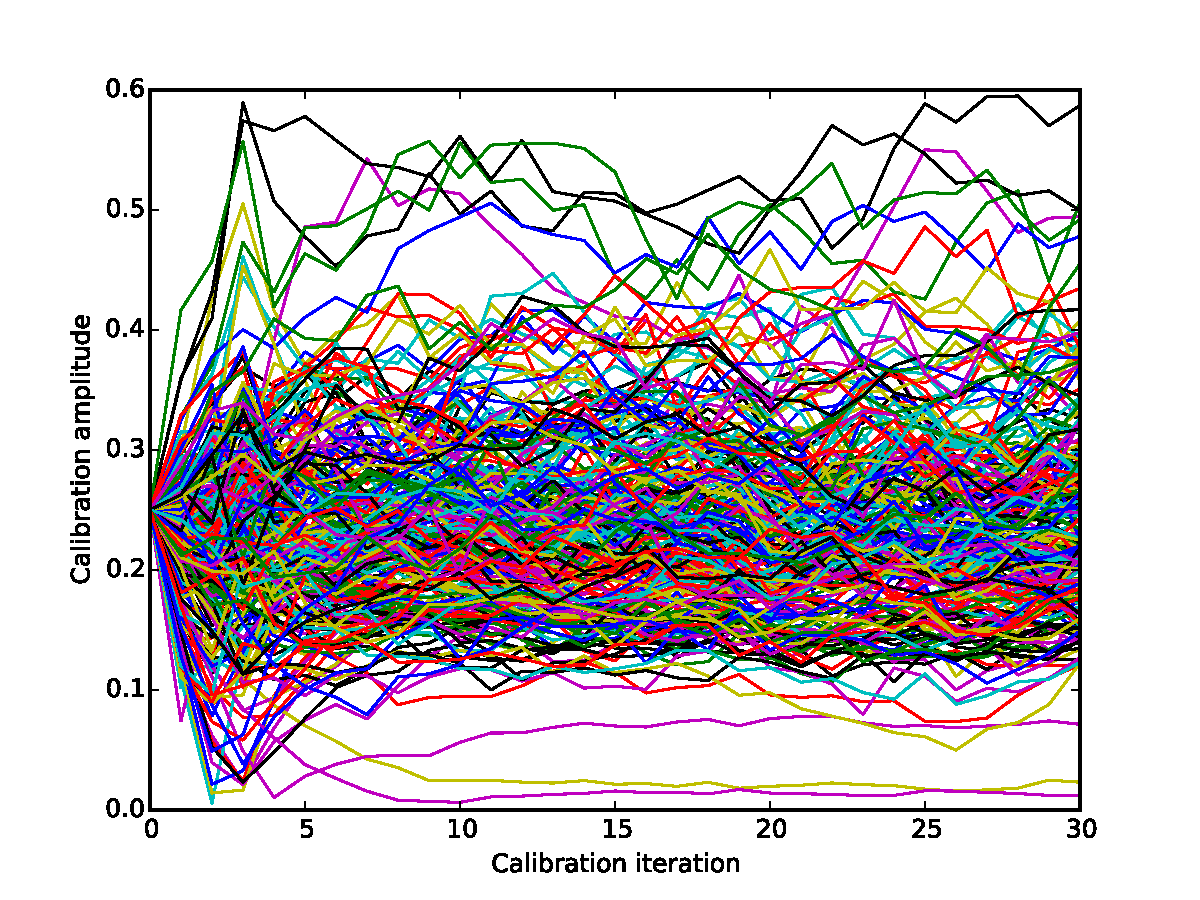
\includegraphics[width=\columnwidth]{fig7.pdf}
\caption{Gain phase solutions as a function of calibration iteration for an LWA TBN observation. 
The gain estimates are initialized with zero phase, but quickly span a $2\pi$ range, and settle 
into relatively flat, albeit noisy, solutions. The majority of phases congregate near zero, which is 
not surprising given the fairly good quality image produced from uncalibrated data.
}
\label{fig:data_phase}
\end{center}
\end{figure}

The gain amplitudes as a function of calibration iteration are shown in 
Fig.~\ref{fig:data_amp}. There is a fairly wide range in gain amplitudes (from 0.12 to 0.59). 
However, this is not surprising due to the non-uniformity in the cables from the antennas to the 
receivers. Again, the amplitudes are noisy but relatively flat.

\textbf{To ensure the level of noise in our solutions is reasonable we compared to the fractional errors
from our simulations shown in Fig.~\ref{fig:errors}. We first use the Global Sky Model
\citep{deo08} to generate a mock observed sky at 74.03 MHz using the PyGSM python 
module\footnote{https://github.com/telegraphic/PyGSM} \citep{pri16}. We integrate this model
to estimate a total sky flux power of 171,000~Jy, meaning our calibration pixel containing
Cyg A accounts for  approximately $20,539/171,000 \approx 12\%$ of the total sky power. 
This places us in a regime similar to the incomplete sky model simulations of the 
previous section, where the calibration pixel accounted for 21.7\% of the sky power. We 
should therefore expect our fractional gain noise levels to be at best around 0.1, the level 
to which the simulations asymptotically approached. }

\textbf{To estimate the fractional gain noise of our solutions we calculate the standard deviation of the gain
estimates after iteration 15 for each antenna separately. We then divide these standard
deviations by the respective mean gain amplitudes. This resulted in a distribution of fractional
gain noise centered at 0.15 and a width of 0.04 ($\approx 0.15/\sqrt{15}$). This noise level
is consistent with what we expected from the simulations.
There were four outliers with noise levels significantly outside the distribution 
($\sigma_g \approx 0.29$). Upon closer inspection the gain amplitudes of these outliers had
converged later in the calibration loop, after iteration 15.}

\begin{figure}
\begin{center}
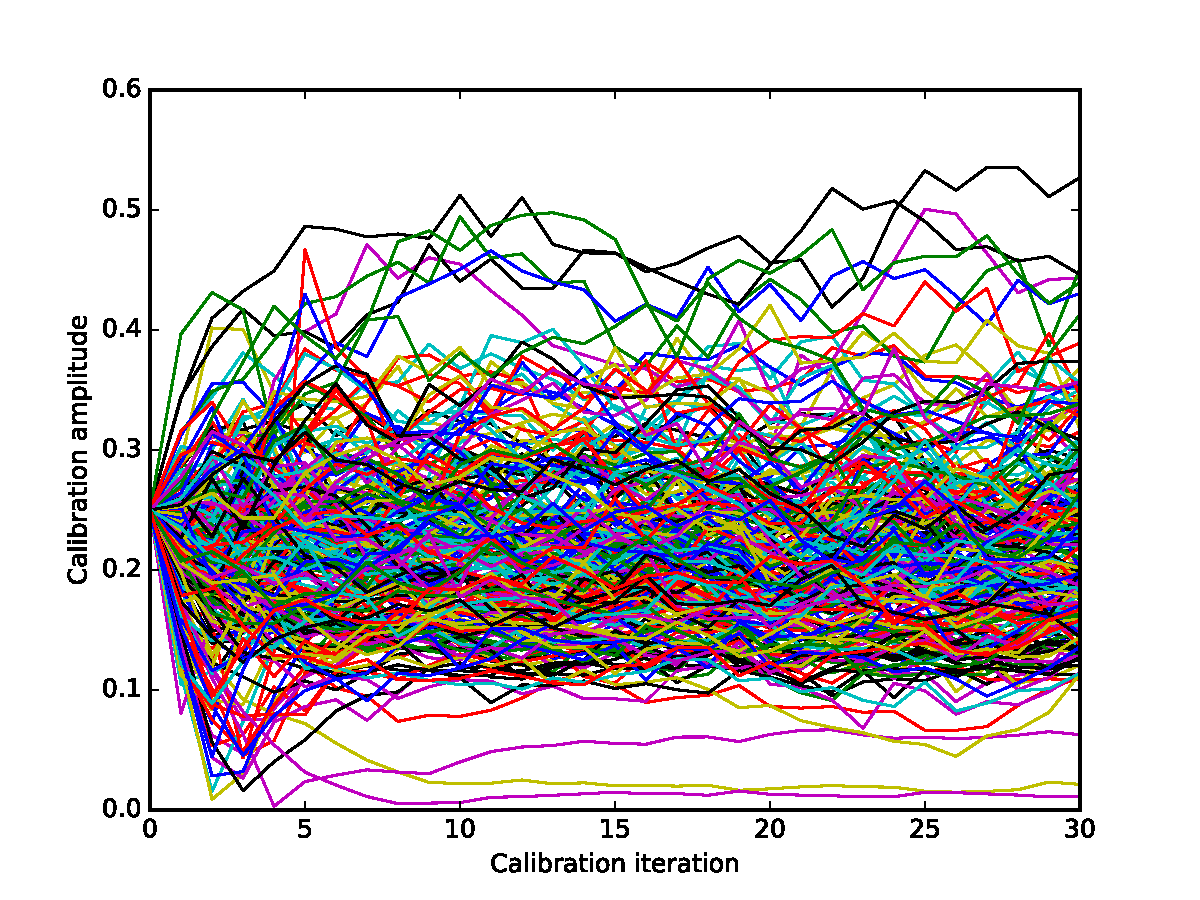
\includegraphics[width=\columnwidth]{fig8.pdf}
\caption{\textbf{Same as Fig.~\ref{fig:data_phase}, but for gain amplitudes.}
The 
gains estimates were initialized with amplitude 0.25 after inspection of the electric field values 
compared to our model sky. The solutions are noisy, but flat. The range in amplitudes is due to 
the non-uniformity of cables between the LWA antennas and receivers.
}
\label{fig:data_amp}
\end{center}
\end{figure}

Figure~\ref{fig:data_images} shows the improvement in the images due to our calibration. The 
left panel shows the uncalibrated image integrated over 51.2 ms, \textbf{58.6 kHz.} Cyg~A is prominent 
near the center of the image, and Cas~A is also clearly visible in the upper right. The middle 
panel shows the image produced after calibration with identical integration time and bandwidth. 
The sidelobes throughout the image are significantly suppressed, and the galactic plane is 
much more evident, despite only modeling Cyg~A and Cas~A. We also note that the feature 
just to the right of Cyg~A is dimmer in the calibrated image, better matching the expected flux 
from the GSM. 
\textbf{For reference we show the GSM in the right panel of 
Fig.~\ref{fig:data_images}, convolved by the LWA point spread function and weighted
by  two factors of the primary beam to match the holographic frame of the data images.}

\begin{figure*}
\begin{center}
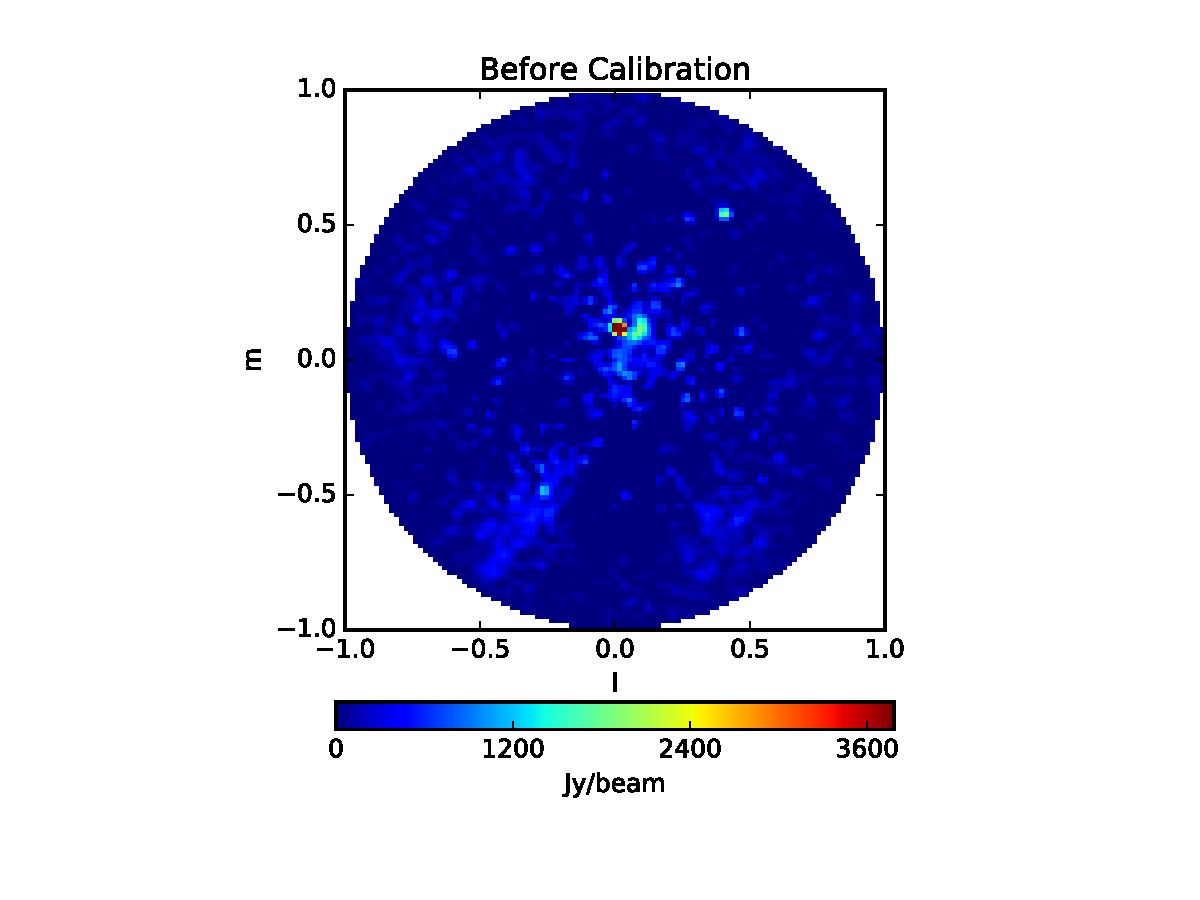
\includegraphics[width=0.3\linewidth]{fig9a.pdf}
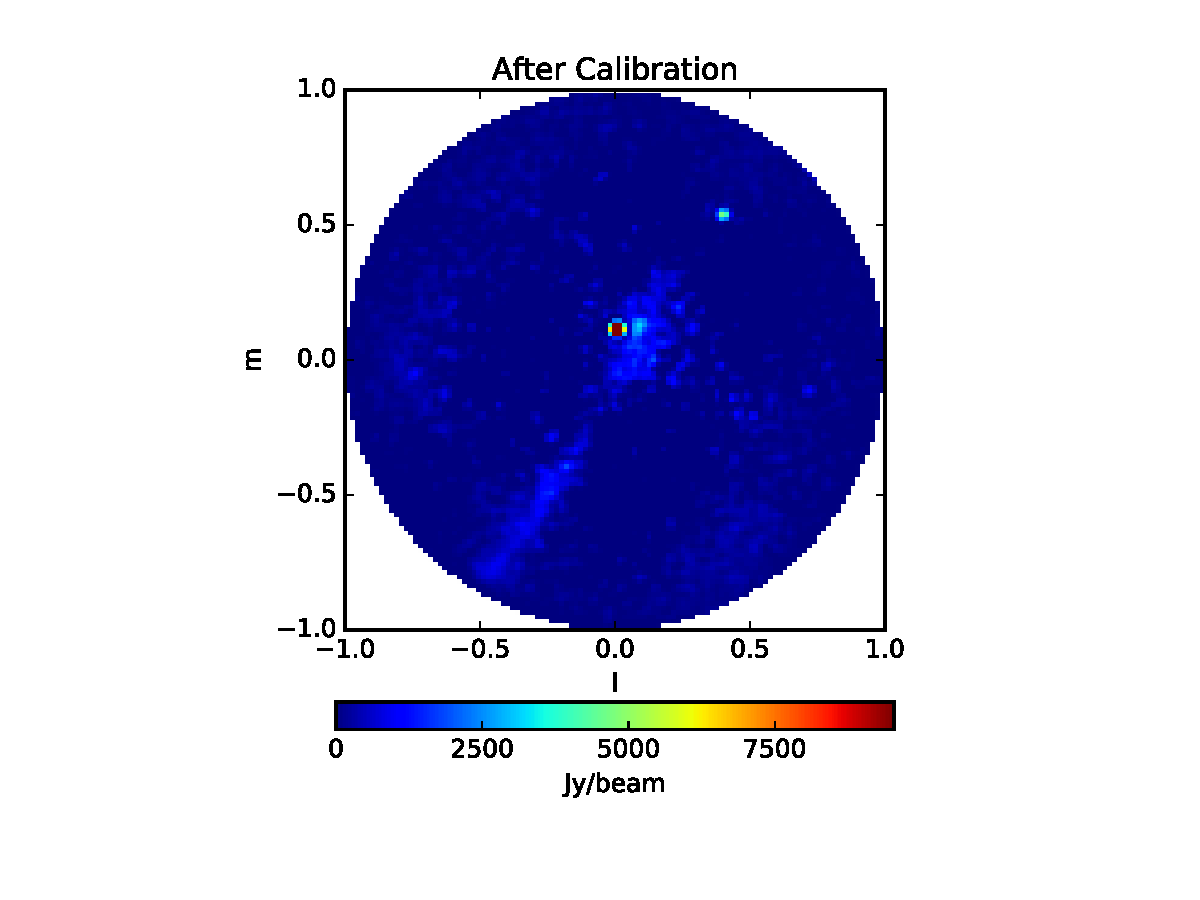
\includegraphics[width=0.3\linewidth]{fig9b.pdf}
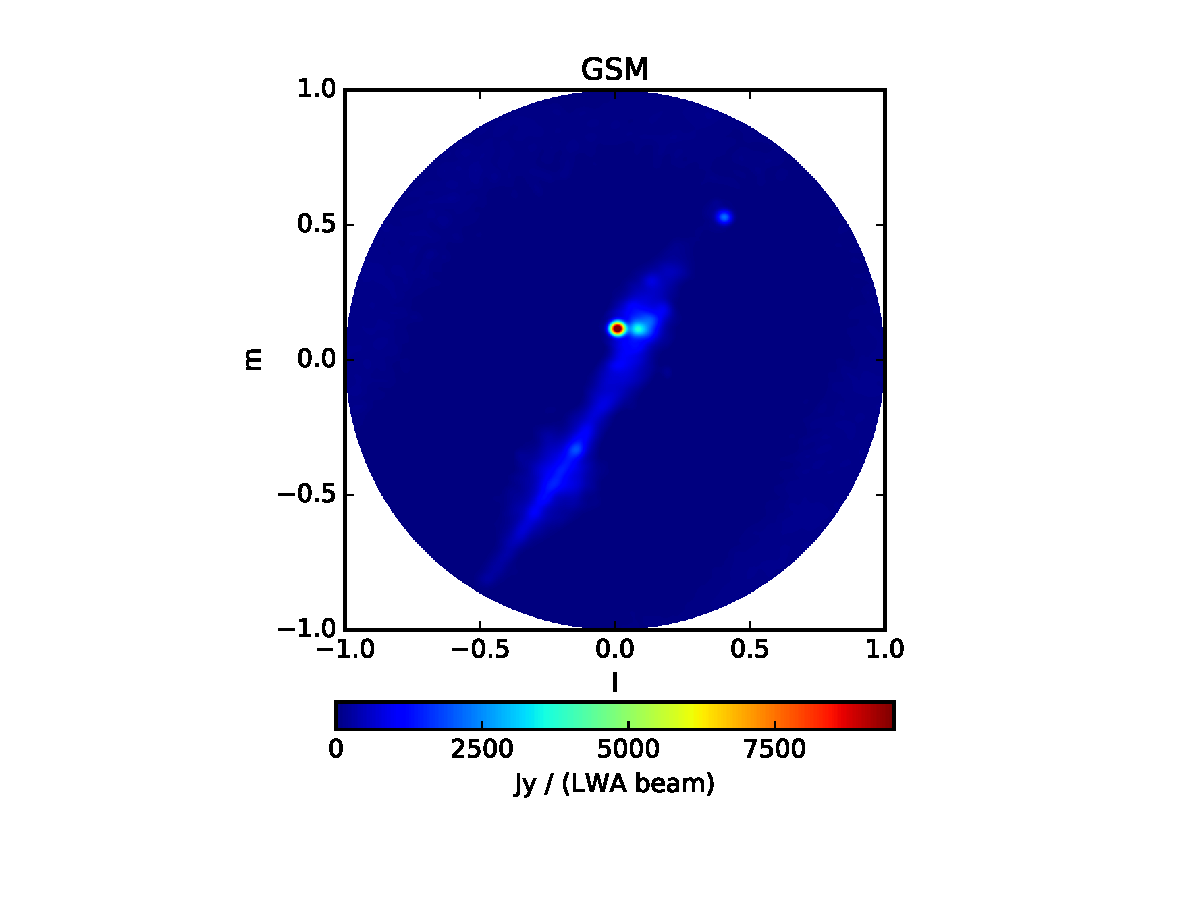
\includegraphics[width=0.3\linewidth]{fig9c.pdf}
\caption{Images produced before (left) and after (middle) calibrating LWA data. These images 
were produced with \textbf{58.6 kHz} bandwidth and 51.2 ms integration. The calibrated image shows 
significant reduction in \textbf{rumble} throughout, while retaining the prominent Cyg~A and 
Cas~A sources. The galactic plane is also substantially more evident after calibration. For 
reference, the GSM is shown \textbf{in the 
right panel convolved with the LWA point spread function and weighted by two factors
of the primary beam to place it in the same holographic frame as the data images.} While much of the GSM is visible in the calibrated image, we 
note that the model used to calibrate was only the two bright sources, Cyg~A and Cas~A.
}
\label{fig:data_images}
\end{center}
\end{figure*}

To compare the image qualities quantitatively we compute the dynamic range, defined as the 
peak of the image over the noise level. We estimate the noise level as the median of the 
absolute deviation of the image. With this metric we find the \textbf{uncalibrated 
and} calibrated images to have \textbf{dynamic ranges of 80.4 and 133.1, respectively, a 65\% 
improvement.}

\section{Discussion}\label{sec:discussion}
Through simulations and application to real data, we have shown that the EPICal algorithm is a 
viable solution for calibrating direct imaging arrays in real time. The computation necessary 
only scales with the number of antenna elements, making it a sub-dominant cost factor when 
designing the correlator. This strategy will enable fast read-out for arrays with many thousands 
of antennas, which will be necessary for future radio transient and cosmology experiments.

EPICal can be further improved through several extensions. Here we name a few potential 
considerations for further study. These topics can be thought of as extensions to the white 
``estimate gains" box in Fig.~\ref{fig:schematic}, which can be performed at a much lower 
cadence than the actual correlations.

\textbf{Multiple pixel correlations.} As was seen in section~\ref{sec:noise}, the single pixel 
correlation demonstrated in this paper can underperform in the presence of a complex sky, 
when compared to visibility-based gains with perfect knowledge of the sky. These errors can be 
mitigated by using correlations of multiple image pixels to incorporate a higher fraction of the 
total sky power into the calibration loop. Of course this increases the computational cost to a 
scaling of $\mathcal{O}(\Nant N_{\mathrm{pix}})$, which will typically be much lower than the 
$\mathcal{O}(\Ng \log_2 \Ng)$ of the correlator itself. These additional correlations would also 
enable direction dependent gain solutions. Each correlation could be used to independently 
solve for gains in each pixel direction, then fit to a beam model on the sky. This updated beam 
pattern would then feed into the gridding step of the correlator, allowing the imager to convolve 
the signals with the effective beam pattern in the ground plane. 

\textbf{Fitting gain models.} With some knowledge of the instrumental bandpass, the noise of 
the gain solutions can be greatly reduced by fitting a model to the per-frequency solutions 
derived here. We used this method at a rudimentary level in our demonstration to LWA data by 
assuming the gains were constant over a narrow bandwidth. One could easily improve on this 
by extending the bandwidth and fitting for a low order polynomial in phase and amplitude. 
Additionally, with knowledge of 
\textbf{any filters applied to the data stream in the receiver chain,}
we could include channels closer to the edge of the band.

\textbf{Improving sky model.} In this work we used a perfect sky model (for simulation), or a 
very simple sky model (for LWA data). In principle the images produced by the EPIC correlator 
can be used to improve the sky model used in calibration -- similar to a major loop in 
self-calibration. This can be especially useful for compact, widefield arrays which require a model of 
both compact and diffuse sources over a large patch of sky. 
\textbf{As with any sky-based calibration scheme, EPICal requires that the sky model be attenuated
by the primary beam,} which 
can be difficult to measure at the precision necessary \citep[e.g.][]{neb15,vir14,thy15b}. 
However, the direct imaging correlator provides exactly the \textbf{product of the sky and beam} necessary in real time, and 
can be iterated over to improve the images and gain solutions, \textbf{leaving final beam
correction to post-processing as in traditional processing.}

\textbf{Dynamic parameters.} In our controlled experiments we fine-tuned a number of 
parameters based on our testing (e.g. damping factor, integration time, frequency averaging). A 
deployed system will require robust determination of these parameters to operate continuously. 
The specifics will be heavily dependent on the stability of the instrument, the frequency of 
observation, and the sky. For example, a stable instrument may be able to use short 
integrations to determine a rough estimate of the gains before switching to much longer 
integration (on order seconds to minutes) to highly increase signal to noise. At low frequencies 
or high imaging resolution, the dynamics of the ionosphere are important, and will likely drive 
the limit of time integration allowed.

The work here will serve as a foundation for further development. We have shown that the 
EPICal algorithm produces reliable calibration solutions, and have identified several aspects to 
increase the scope. With next generation instruments in the planning and development stages, 
EPICal is poised to \textbf{enable new design spaces}. The software is integrated into the EPIC 
package and freely available to use in simulations or \textbf{post-processing} of data. Work is 
underway to port the code to real-time GPU systems for deployment. 

\section*{Acknowledgements}
This work has been supported by the National Science Foundation through award 
AST-1206552. We thank Danny Jacobs for his valuable inputs, and Greg Taylor for providing 
us with LWA data. Construction of the LWA has been supported by the Office of Naval 
Research under Contract N00014-07-C-0147. Support for operations and continuing 
development of the LWA1 is provided by the National Science Foundation under grant 
AST-1139974 of the University Radio Observatory program.



%%%%%%%%%%%%%%%%%%%% REFERENCES %%%%%%%%%%%%%%%%%%

% The best way to enter references is to use BibTeX:

\interlinepenalty=10000
\bibliographystyle{../mnras}
\bibliography{../epic} % if your bibtex file is called example.bib
%
% Basic setup. Most papers should leave these options alone.
\documentclass[a4paper,fleqn,usenatbib]{../mnras}

\usepackage{newtxtext,newtxmath}

% Use vector fonts, so it zooms properly in on-screen viewing software
% Don't change these lines unless you know what you are doing
\usepackage[T1]{fontenc}
\usepackage{ae,aecompl}


%%%%% PACKAGES %%%%%

% Only include extra packages if you really need them. Common packages are:
\usepackage{graphicx}	% Including figure files
\usepackage{amsmath}	% Advanced maths commands
\usepackage{amssymb}	% Extra maths symbols
\usepackage{color}

%%%%% CUSTOM COMMANDS %%%%%

\newcommand{\Nant}{\ensuremath{N_{\mathrm{a}}}}
\newcommand{\Ng}{\ensuremath{N_{\mathrm{g}}}}
\newcommand{\s}{\ensuremath{\hat{\mathbf{s}}}} % s-hat for sine-projected direction
\newcommand{\spix}{\ensuremath{\hat{\mathbf{s}}_{0}}}
\newcommand{\Cna}[1][n]{\ensuremath{\mathcal{C}^{(#1)}_{a,\spix}}}
\newcommand{\ri}{\ensuremath{\mathbf{r}_i}}
\newcommand{\ra}{\ensuremath{\mathbf{r}_a}}
\newcommand{\rb}{\ensuremath{\mathbf{r}_b}}
\newcommand{\beamr}{\ensuremath{\widetilde{W}}}
\newcommand{\beamtheta}{\ensuremath{W}}
\newcommand{\Er}[1]{\ensuremath{\widetilde{E}_{#1}}}
\newcommand{\Erest}[1]{\ensuremath{\widetilde{E}'_{#1}}}
\newcommand{\Ethetaest}{\ensuremath{E'}}
\newcommand{\V}{\ensuremath{\widetilde{V}}}
\newcommand{\dif}{\mathrm{d}}
\newcommand{\caliter}{400}
\newcommand{\damp}{\ensuremath{\gamma}}
\newcommand{\itr}{20}

%%%%%%%%%%%%%%%%%%% TITLE PAGE %%%%%%%%%%%%%%%%%%%

% Title of the paper, and the short title which is used in the headers.
% Keep the title short and informative.
\title[E-field Parallel Imaging Calibration]{An Efficient E-field Parallel Imaging Calibration Algorithm for Next-Generation Radio Telescopes}

% The list of authors, and the short list which is used in the headers.
% If you need two or more lines of authors, add an extra line using \newauthor
\author[Beardsley et al.]{
Adam P. Beardsley,$^{1}$\thanks{E-mail: Adam.Beardsley@asu.edu}
Nithyanandan Thyagarajan,$^{1}$
Judd D. Bowman$^{1}$
\newauthor
and Miguel F. Morales$^{2}$
\\
% List of institutions
$^{1}$Arizona State University, School of Earth and Space Exploration, Tempe, AZ 85287, USA\\
$^{2}$University of Washington, Department of Physics, Seattle, WA 98195, USA\\
}

% These dates will be filled out by the publisher
\date{Accepted XXX. Received YYY; in original form ZZZ}

% Enter the current year, for the copyright statements etc.
\pubyear{2015}

% Don't change these lines
\begin{document}
\label{firstpage}
\pagerange{\pageref{firstpage}--\pageref{lastpage}}
\maketitle

% Abstract of the paper
\begin{abstract}
Abstract here (250 words)
\end{abstract}

\begin{keywords}
instrumentation: interferometers -- techniques: image processing -- techniques: interferometric
\end{keywords}


%%%%%%%%%%%%%%%%% BODY OF PAPER %%%%%%%%%%%%%%%%%%

\section{Introduction}
In order to satisfy the survey speeds required for precision cosmology as well as searches for fast radio transients, radio astronomy is undergoing a paradigm shift toward interferometers consisting of hundreds to thousands of small, widefield antennas. Many arrays with this design are already built or under construction including the Hydrogen Epoch of Reionization Array\footnote{http://reionization.org} (HERA), the Murchison Widefield Array (MWA;\citealt{tin13,bow13}), the Precision Array for Probing the Epoch of Reionization (PAPER; \citealt{par10}), the LOw Frequency ARray (LOFAR; \citealt{van13}), the Canadian Hydrogen Intensity Mapping Experiment (CHIME,\citealt{ban14}), the Long Wavelength Array (LWA, \citealt{ell13}), and the low frequency Square Kilometer Array (SKA1-Low \citealt{mel13}).

Traditional radio correlators cross-multiply the voltage signals from all pairs of antennas, and the computation scales as the number of antennas squared, $\mathcal{O}(\Nant^2)$ \citep{bun04}. As the number of elements in future arrays grows, the computational cost will become prohibitively expensive, and exploring efficient correlator schemes is essential to enable next generation instruments \citep{lon00}. Meanwhile, radio transient monitoring requires access to high time and frequency resolution data. For example, fast radio bursts (FRBs) are highly unexplored at low frequencies (< 1 GHz), but are expected to occur on timescales $\Delta t \sim$ 1--10~ms \citep{tho13}. Recording the full visibility matrix for $\Nant \gtrsim 10^3$ arrays at this timescale leads to extremely high data write rates. 

Direct imaging correlators are a new variety of radio correlator which aim to alleviate both the computational strain of forming $\Nant^2$ correlations and the high data throughput associated with short timescale science. This is done by performing a spatial fast Fourier transform (FFT) to image the antenna voltages, then squaring and averaging in time. This process scales as $\mathcal{O}(\Ng \log_2 \Ng)$, where \Ng~is the number of grid points in the FFT \citep{mor11, teg09, teg10}. For certain classes of telescopes, significantly those envisioned for next generation cosmology experiments, this scaling is a large improvement over the $\Nant^2$ scaling of traditional methods. Furthermore, because images are generated online, the native output bandwidth will be lowered (assuming $\Ng < \Nant^2$), and has the potential to be lowered even further with online transient processing.

A handful of prototype direct imaging correlators have been tested on arrays including the Basic Element for SKA Training II (BEST-2) array \citep{fos14}, the Omniscope \citep{zhe14}, and an earlier pulsar timing experiment at GHz frequencies \citep{oto94, dai00}. Each of these are examples of so-called FFT correlators -- a subclass of direct imaging correlators which rely on identical antennas with restricted placement, which allows the FFT to be performed without gridding. We recently released the E-field Parallel Imaging Correlator \citep[EPIC;][]{thy15c}, which is a software implementation of the Modular Optimal Frequency Fourier \citep[MOFF;][]{mor11} imaging algorithm. This architecture leverages the software holography/A-transpose framework to grid electric field data streams before performing the spatial FFT, allowing for an optimal map without placing constraints on array layout or requiring identical antennas \citep{mor09,bha08,teg97a}.

A challenge common to all direct imaging algorithms is calibration of the antenna gains. Traditionally, pair-wise visibilities are written to disk and used to calibrate offline. However, a direct imaging correlator mixes the signals from all antennas before averaging and writing to disk, making calibration a requirement at the front end. Previous solutions have involved applying calibration solutions generated from a parallel FX correlator \citep{zhe14, fos14}, or integrating a dedicated FX correlator which periodically formed the full visibility matrix to solve for gains \citep{wij09,dev09}. While these solutions were sufficient to enable the exploration of FFT correlators and beamformers, they will not scale to future arrays with $\Nant \gtrsim 10^3$.

Here we present the E-field Parallel Imaging Calibration (EPICal) algorithm -- a novel solution to the calibration problem, which can be integrated into direct imaging correlators and scales only as the number of antennas, $\mathcal{O}(\Nant)$. This method uses a correlation of the uncalibrated antenna signal stream with an output image pixel from the backend of the correlator to solve for the complex gains of the antennas. Because the calibration must be applied before gridding and imaging, our solution requires an iterative approach where the data from one time series is used to update the gains which are applied to the following time series. An example implementation of the algorithm is available with the EPIC software package\footnote{http://github.com/nithyanandan/EPIC}.

We establish the mathematical framework and derive the calibration algorithm in \S \ref{sec:math}. We then demonstrate the algorithm in simulations in \S \ref{sec:sim}, and apply to a sample LWA data set in \S \ref{sec:data}. Then we discuss the noise properties of the resulting gain solutions in \S \ref{sec:noise}. Finally we conclude and discuss potential extensions to the algorithm in \S \ref{sec:discussion}.

\section{Mathematical Framework}\label{sec:math}
We begin by establishing the mathematical framework for the calibration problem. We derive the calibration solutions for the MOFF algorithm (adopting the notation of \citealt{thy15c}), but note the result is easily extended to FFT correlator algorithms by removing the gridding step.

The electric field incident on the ground, $\Er{}(\mathbf{r},f,t)$, is related to the sky electric field, $E(\hat{\mathbf{s}},f,t)$, through a Fourier transform.
\begin{equation}
\Er{}(\mathbf{r},f,t) = \int E(\hat{\mathbf{s}},f,t) e^{-2\pi i \mathbf{r}\cdot \hat{\mathbf{s}}}\, \dif^2 \hat{\mathbf{s}}
\end{equation}
Here $\hat{\mathbf{s}}$ denotes the sine-projected unit vector for the sky angle, $\mathbf{r}$ is the observer's location (measured in wavelengths relative to an arbitrary origin), and $f$ and $t$ denote the frequency and time dependence, respectively. We will encounter several quantities which we attempt to estimate. We distinguish the ``true" values with a superscript $T$, while the estimates are denoted with a prime. We define the true antenna signal as a convolution of the antenna voltage pattern, $\beamr$, with the electric field on the ground.
\begin{equation}
\Er{a}^T(f,t) \equiv \int \beamr_a(\mathbf{r}-\ra) \Er{}(\mathbf{r},f,t) \, \dif^2 \mathbf{r}
\end{equation}
The subscript $a$ labels the antenna, and $\mathbf{r}_a$ is the location of antenna $a$.

We next model the measured, uncalibrated electric field as a multiplicative complex gain and an additive noise term applied to the true antenna electric field. 
\begin{equation}\label{eq:apply_gain}
\Er{a}(f,t) = g^T_a(f,t) \Er{a}^T(f,t) + \widetilde{n}_a(f,t)
\end{equation}
Note that this quantity is neither a true or estimated value. The noise term is strictly receiver noise -- noise introduced by the instrument. Any sky noise is implicitly included in the time dependence of the sky electric field. As the noise of modern low frequency arrays is heavily dominated by sky noise, we will neglect $\widetilde{n}_a$ for now, but will inspect its effects at the end of this section.

The goal of our calibration algorithm will be to estimate the antenna gains. We will assume the gains have no time dependence within the timescale of finding our solutions. \textcolor{red}{cite someone about gain stability}. Furthermore, we will treat each frequency channel independently, and drop the $f$ to simplify notation.

The MOFF algorithm next calls for a calibration. We will assume we have formed an estimate of the gains after $n$ iterations of a calibration loop, and derive an updated $n+1$ estimate. Typically calibration amounts to dividing the measured fields by the gain (in the case of sky noise dominance), or multiplying by the complex conjugate of the gain (receiver noise dominance). We will abstain from this choice for now, and instead use a multiplicative factor $h^{(n)}_a$ to represent the application of our $n^{\mathrm{th}}$-loop estimate of the gain for antenna $a$:
\begin{equation}
\Erest{a} = h^{(n)}_a \Er{a}
\end{equation}
where,
\begin{equation}
h^{(n)}_a=\begin{cases}
1/g^{(n)}_a & \mbox{sky noise dominated} \\ 
g^{*(n)}_a & \mbox{receiver noise dominated}.
\end{cases}
\end{equation}

A dirty image is next formed by gridding the calibrated fields with the antenna voltage pattern, Fourier transforming, squaring, and averaging in time. The estimated value for a pixel, $\s_i$, can be expressed as
\begin{equation}
I'(\s_i) = \left<\left| \frac{1}{\Nant}\sum_i e^{2\pi i \mathbf{r}\cdot \s_i} \sum_a \beamr_a(\ri - \ra) h^{(n)}_a g^T_a \Er{a}^T(t) \right|^2 \right>_t.
\end{equation}
This is the final output of the MOFF correlator. However, for calibration purposes we will be interested in the electric field image just prior to squaring and averaging.
\begin{equation}
\Ethetaest (\s_i,t) = \frac{1}{\Nant} \sum_i e^{2\pi i \ri \cdot \s_i} \sum_a \beamr_a(\ri - \ra) h^{(n)}_a g^T_a \Er{a}^T(t)
\end{equation}
We can simplify this expression by exchanging the sums to transform the beam term into sky coordinates.
\begin{align}\label{eq:epix}
\Ethetaest(\s_i,t) & = \frac{1}{\Nant} \sum_a h^{(n)}_a g^T_a\Er{a}^T(t) e^{2\pi i \s_i \cdot \ra}\sum_i \beamr_b(\ri-\ra)e^{2\pi i \s_i \cdot (\ri-\ra)} \nonumber\\
& = \frac{1}{\Nant} \sum_a h^{(n)}_a g^T_a\Er{a}^T(t) e^{2\pi i \s_i \cdot \ra}\beamtheta_a(\s_i)
\end{align}

Next we move toward the feedback calibration outlined in \citealt{mor11}. The calibration loop described there assumed a simple sky of a single point source, but we aim for a more generalized solution for arbitrarily complex sky models. As such the quantity we wish to inspect is a correlation of the uncalibrated antenna signals input to the correlator with the holographic electric field image output from the correlator. We define the quantity,
\begin{equation}\label{eq:Cna}
\Cna \equiv \left<\Er{a}(t) E'^*(\spix,t)\right>_t,
\end{equation}
where the superscript $n$ again represents the quantity formed in the $n^\mathrm{th}$ calibration loop, and \spix\, is the pixel center nearest a bright calibrator of interest. The following will hold for any chosen pixel, \spix, though it is advantageous to choose a pixel which contains a bright source to achieve a high signal to noise. 

Plugging equation \ref{eq:epix} into equation \ref{eq:Cna}, we find,
\begin{align}\label{eq:cna}
\Cna & = \left<g^T_a \Er{a}^T(t) \frac{1}{\Nant} \sum_b h^{*(n)}_b g^{T*}_b\Er{b}^{T*}(t) e^{-2\pi i \spix \cdot \rb} \beamtheta^*_b(\spix)\right>_t \nonumber \\
& = \frac{g^T_a}{\Nant} \sum_b h^{*(n)}_b g^{T*}_b \beamtheta^*_b(\spix) e^{-2\pi i \spix \cdot \rb} \left<\Er{a}^T \Er{b}^{*T} \right>_t \nonumber \\
& = \frac{g^T_a}{\Nant} \sum_b h^{*(n)}_b g^{T*}_b \beamtheta^*_b(\spix) e^{-2\pi i \spix \cdot \rb} \V^T_{ab}
\end{align}
where in the second step we group time-dependent terms, and in the third we define the true visibilities as the correlation between true antenna electric field measurements. It is easy to see from here that the net effect of including the receiver noise term, $\widetilde{n}_a(f,t)$, will result in added noise on the true visibilities. In principle this can include any noise correlations between antennas. The implementation included in the EPIC software package restricts the noise term to include only the auto-correlation noise bias, and assumes baseline dependent noise is zero mean.

Finally, we find an update to our gain solution by assuming our current estimate of the gains, $g^{(n)}_b$, is approximately correct and substitute into the sum for the true gains. We also require model visibilities formed from sky and primary beam models in place of true visibilities.
\begin{equation}\label{eq:cal_solution}
g'^{(n+1)}_a = \Cna \Nant \left[ \sum_b h^{*(n)}_b g^{*(n)}_b \beamtheta^*_b(\spix) e^{-2\pi i \spix \cdot \rb} \V^T_{ab} \right]^{-1}
\end{equation}
This equation is our prescription for estimating the antenna gains of a direct imaging array. The approach is iterative in nature, and requires a sky model. However, the sky model can be precomputed offline, and the online computation complexity scales only as $\mathcal{O}(\Nant)$ as we form a $\Cna$ for each antenna. In the case where $h_b = 1/g_b$ (typical calibration procedure for sky-noise dominated systems), this simplifies slightly.
\begin{equation}\label{eq:cal_solution_simple}
g'^{(n+1)}_a = \Cna \Nant \left[ \sum_b \beamtheta^*_b(\spix) e^{-2\pi i \spix \cdot \rb} \V^T_{ab} \right]^{-1}
\end{equation}

While testing we found equation~\ref{eq:cal_solution} resulted in oscillatory gain solutions as it was iterated, as is often the case in iterative minimization methods. To mitigate this we introduce a damping factor, $0 \leq \damp <1$, which is used to attenuate the gain update, effectively giving the solutions memory of previous iterations.
\begin{equation}
g^{(n+1)}_a = (1-\damp) g'^{(n+1)}_a + \damp g^{(n)}_a
\end{equation}
We found that while equation~\ref{eq:cal_solution} does indeed converge on good solutions, the process is faster by tuning the damping factor. We note the small difference between $g^{(n+1)}_a$ and $g'^{(n+1)}_a$, where the prime indicates our current best estimate of the true gain, while no prime is actually used in the iterative calibration loop. Once the loop converges the difference is a longer effective integration for the non-primed version (lower thermal noise). 

We show schematically the process of calibrating a direct imaging correlator in figure~\ref{fig:schematic}. Computationally expensive steps that must be performed ``on-chip" are shown inside the gray box. The uncalibrated antenna signals are tapped out after the F-engine and correlated against the output image pixel of interest. The correlated values are then passed off-chip to estimate the gains using equation~\ref{eq:cal_solution}, and additional fitting if desired. The gains are then passed back to the correlator to update the calibration for subsequent data streams. 

\begin{figure}
\begin{center}
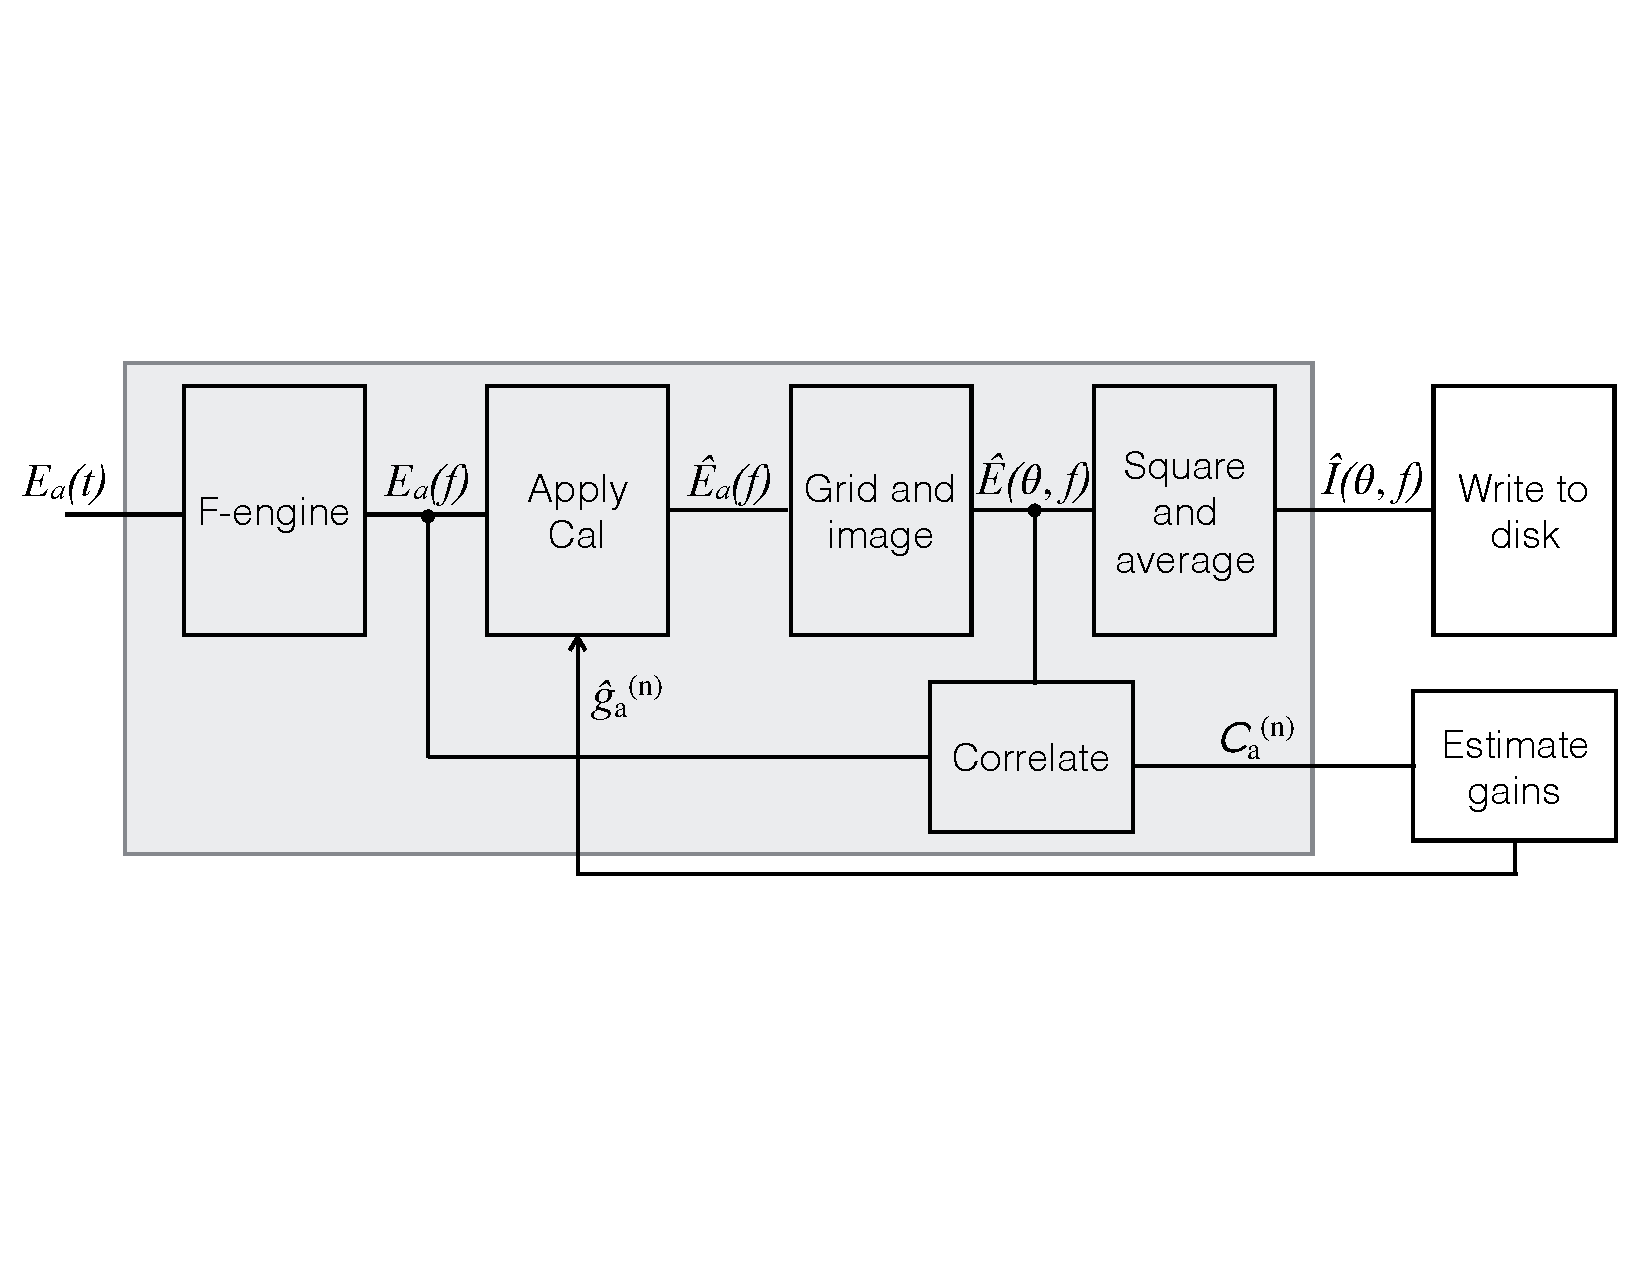
\includegraphics[width=\columnwidth]{figures/schematic.pdf}
\caption{The general data flow of the MOFF correlator, with a feedback calibration loop. A pixel from the (unsquared) image is tapped out and correlated against the input antenna electric field signals to form $\Cna$ coefficients, which are used to estimate the antenna gains. These gain estimates are then fed back into the correlator to be applied to subsequent data, and the process is repeated. The gray box shows operations which must be done at high speed (before averaging in time), which white boxes show operations which can be performed ``off-chip".}
\label{fig:schematic}
\end{center}
\end{figure}

An important feature to note is that, like the MOFF-generated images themselves, equations~\ref{eq:cal_solution} and~\ref{eq:cal_solution_simple} include the antenna auto-correlations (the sum is over \emph{all} $b$, not excluding $a$). It can be difficult to perfectly model the noise bias from auto-correlations, which can often times be far brighter than the visibilities themselves. It can therefore be beneficial to subtract this term directly from \Cna, and exclude the $b=a$ term in the sum.
\begin{equation}
\Cna \rightarrow \Cna - \frac{1}{\Nant} h^{*(n)}_a\beamtheta^*_a e^{-2\pi i \spix \cdot \ra} \left<|\Er{a}|^2\right>_t
\end{equation}
This requires generating these correlations, which again only scale as $\mathcal{O}(\Nant)$, and are generally useful for array diagnostics.

We conclude this section by connecting our calibration expression to that found in a visibility framework. In the limit of a single bright calibrating source at phase center, we can greatly simplify equations~\ref{eq:cna} and~\ref{eq:cal_solution}. We will assume the beams are normalized such that $\beamtheta(0)=1$. We can further drop the exponential phase terms because $\spix=0$. We then absorb the true gains and gain corrections into the true visibilities in equation~\ref{eq:cna} to express as a sum of measured visibilities.
\begin{equation}
\mathcal{C}^{(n)}_{a,0} \rightarrow \frac{1}{\Nant}\sum_b h^{*(n)}_b \V_{ab}
\end{equation}

We next plug this expression into equation~\ref{eq:cal_solution} to find our simplified calibration solution for a single bright point source. Because our sky is a single bright point source, the model visibilities are simply the flux of the source, $S_{\mathrm{src}}$.
\begin{equation}
g'^{(n+1)}_a \rightarrow \left[\sum_b h^{*(n)}_b \V_{ab}\right] \times \left[S_{\mathrm{src}}\sum_b h^{*(n)}_b g^{*(n)}_b\right]^{-1}
\end{equation}
This is simply a gain-weighted sum of the measured visibilities over the flux of the source, which is indeed the limiting result from a visibility approach, for example seen in \citealt{mit08}. The ability to recover the equivalent expression despite not actually forming the visibilities is a result of the fact that only sums over visibilities come into the FX solution, as was described in \citealt{mor11}. We have confirmed the limiting case equivalence here, and will explore the more general case in more detail in \S~\ref{sec:noise}.


\section{Simulation}\label{sec:sim}
We first demonstrate our calibration method through a controlled simulation. A complex gain is created for each antenna with random phase and amplitude, which is used to corrupt the simulated data stream, then we attempt to recover the gains using our calibration routine. The simulation software used is included in the EPIC package.

Our simulated signal consists of 10 random point sources with flux densities 0.5~Jy~$\lesssim S \lesssim 1$~Jy. For an antenna array we use the inner 51 antennas of the MWA layout \citep{bea12}, within a bounding box of 150~m. The antenna voltage pattern used is a 4.4~m square tophat on the ground. Because our algorithm treats frequency channels independently, we simulate only one channel. For context we treat this channel as a single 40 kHz, meaning each subsequent timestep is separated by 25~$\mu$s.

For our unknown gains, we create a set of random numbers with amplitude $1\pm0.25$, and completely random phase. These are our ``true gains", and we apply them to the frequency-domain simulated antenna electric fields as in equation~\ref{eq:apply_gain}. Our analysis is blind to these values until the end of the process to check accuracy. The gain estimates are initialized with unity, $g^{(0)}_a=1$.

We next process and image \caliter~time steps (10~ms). We also form the correlations, \Cna[0], used in our calibration loop. The pixel used for the correlation is the source with the largest apparent flux (intrinsic flux attenuated by the primary beam). These correlation values are used to update the gain estimates, which in turn are used to calibrate the following \caliter~time steps. Through experimentation we found a damping factor of $\damp=0.35$ resulted in the quickest convergence in this simulation.

The calibration loop continues by updating the gain estimates every \caliter~time steps. The phases of our gain estimates are shown in figure~\ref{fig:sim_phase} for 20 such iterations. The phase error plotted is the phase relative to the true gain for each antenna (various colored lines). One antenna was used as a reference to fix the absolute phase, so has zero phase error. The other 50 antennas are shown to have error spanning $2\pi$ initially, and after about 10 iterations lock into a solution, settling down to noise levels around iteration 15 (0.15~s). We stop the simulation when the updated gains trace the thermal noise of the simulated sources, which can be seen by the coherence of the 50 antenna gains after iteration 15.

\begin{figure}
\begin{center}
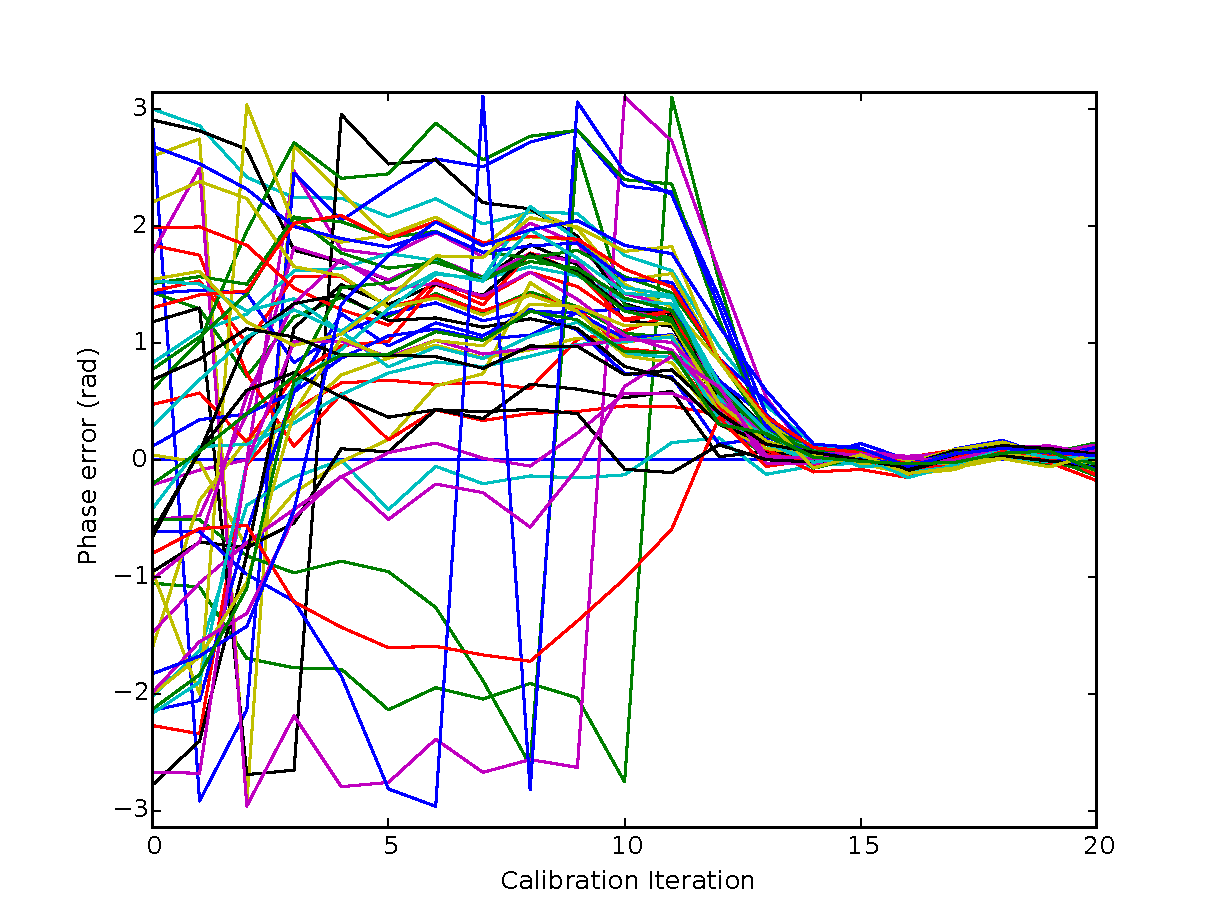
\includegraphics[width=\columnwidth]{figures/cal_paper_sim_phase.pdf}
\caption{Phase error of gain estimates as a function of iteration for simulated calibration. The gains were initialized with random phases, but the calibration loop was able to recover the correct phases after about 15 iterations. Each line represents an antenna in our 51 MWA antenna sample.
}
\label{fig:sim_phase}
\end{center}
\end{figure}

The estimated gain amplitudes for the simulations are shown in figure~\ref{fig:sim_amp}. The quantity plotted is the magnitude of the estimated gains over the true gains, $\left|g^{(n)}_a/g^T_a\right|$, which places all antennas on the same scale. We can see the amplitudes converge toward their true values around the same time as the phases (iteration $\sim$15). At the beginning of calibration we can see the value of the damping factor. At $n=0$, a couple of gains are shown to have abnormally high amplitude estimates, notably one about 3.3 times its true value (red line). These unbalanced high estimates caused the entire set of gains to be under estimated at $n=1$, even with a damping factor of 0.35. By $n=5$ the unbalanced amplitudes have been damped out and the calibration continues. Without the damping factor, the oscillation seen in the first couple iterations would have been significantly larger and taken much longer to fade out.

\begin{figure}
\begin{center}
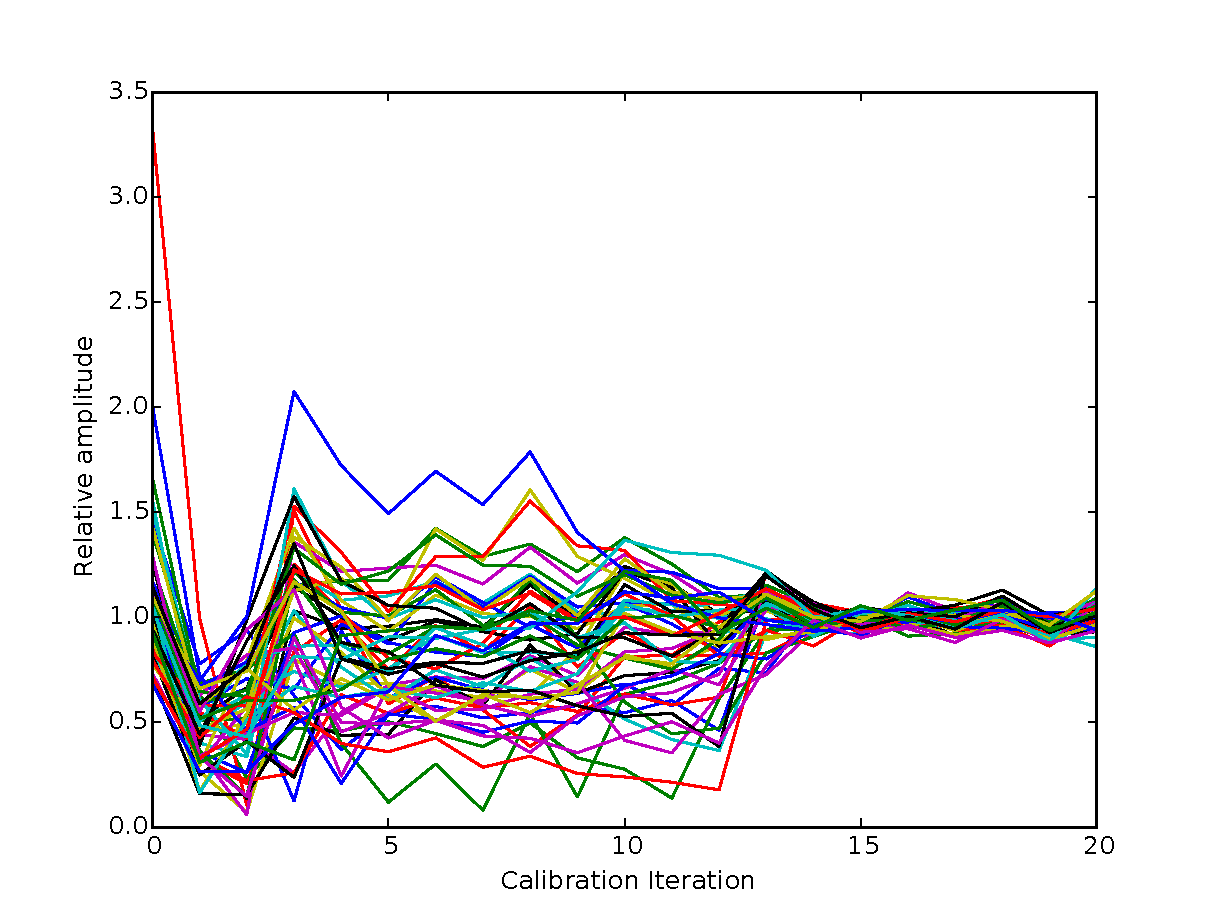
\includegraphics[width=\columnwidth]{figures/cal_paper_sim_amps.pdf}
\caption{Gain estimate amplitudes as a function of iteration for simulated calibration. Again, each line represents an antenna in the 51 MWA antenna sample. The gain estimates were initialized randomly, while the true values were unity. After about 15 iterations we see the calibration loop has settled around the correct values, with only noise remaining.}
\label{fig:sim_amp}
\end{center}
\end{figure}

Images created at the beginning of calibration and at the end are shown in figure~\ref{fig:sim_images}. Each image is 10~ms integration, corresponding to all snapshot images created with a given set of gain estimates. The top panel shows the image produced with our initialized unity gains. Because the phases are completely random, the image is essentially noise with the primary beam evident. After 20 iterations, the image is far more clear, shown in the bottom panel. Each of the ten simulated sources are clearly visible, indicated with red circles. 



\begin{figure}
\begin{center}
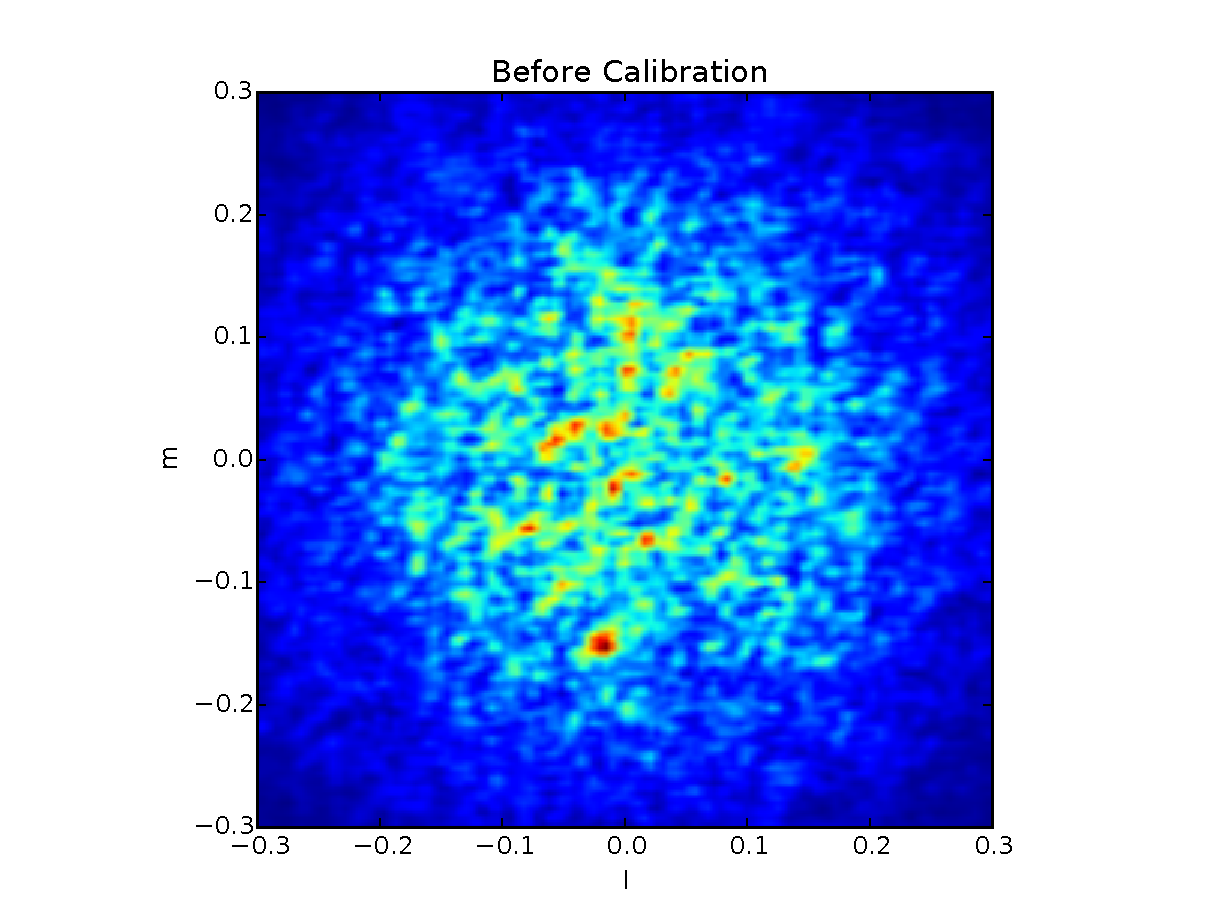
\includegraphics[width=\columnwidth]{figures/cal_paper_sim_image_before.pdf}
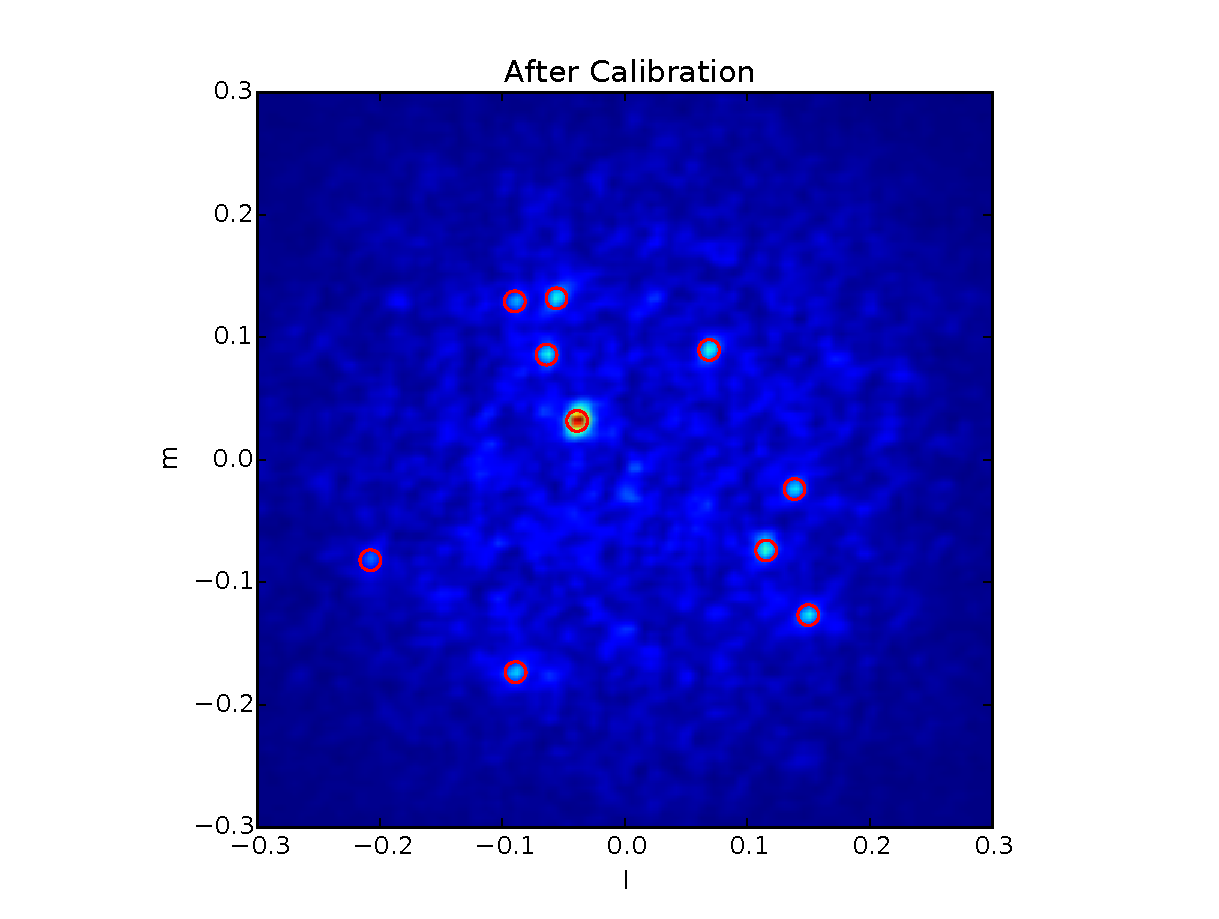
\includegraphics[width=\columnwidth]{figures/cal_paper_sim_image_after.pdf}
\caption{Images formed during simulated calibration. \emph{Top:} An image generated from a single frequency channel and 10 ms integration after the gain estimates are randomized. As expected with random phases, the image is completely noisy, with the shape of the primary beam evident. \emph{Bottom:} An image formed after calibration, again with a single frequency channel and 10 ms integration. The ten simulated (and modeled) point sources are easily visible, and highlighted with red circles.
}
\label{fig:sim_images}
\end{center}
\end{figure}

\section{Application to LWA data}\label{sec:data}
We next demonstrate our calibration algorithm using an observation from the LWA station in New Mexico. The data is from the LWA narrow-band transient buffer (TBN), with time ordered voltage data from 255 antennas within a core radius of 100~m. The central frequency is 74.03 MHz, and a bandwidth of 100 kHz and writeout timescale of 5.12 ms (frequency channel resolution of 195.3125 Hz). For this demonstration we limit ourselves to a single polarization.

After correcting for geometric cable delays, the instrument is naturally well calibrated, as was seen in the demonstration of the EPIC imager in \citealt{thy15c}. However, we will aim to improve yet on this calibration using our algorithm.

We proceed by forming model visibilities. We model only two bright objects as point sources: Cyg A with flux 16611.68 Jy \citep{coh07}; and Cas A with flux 17693.9 Jy \citep{kas07}. Because the raw data is attenuated by the primary beam of the instrument, we also account for this in our model using beam values consistent with \cite{hic12}.

We made several choices while studying the behavior of the LWA data to improve our calibration. We inspected the amplitudes of the voltages to be roughly consistent with average gain amplitudes of 0.25, so we initialized our gains at this level to allow the calibration to converge quickly. We also found a boost in signal to noise is achieved easily by averaging frequency channels and assuming the gains are constant within a sub-band. Here we average solutions across 150 channels, or about 29 kHz. With a fractional bandwidth $B/f_0 = 3.9 \times 10^{-4}$, we felt safe assuming a smooth bandpass. Because there is still a fair amount of noise in the data, a damping factor of $\gamma = 0.7$ was adopted.

Finally, we found that seven antennas\footnote{LWA antenna IDs 48, 85, 124, 148, 203, 217, and 244 were flagged.} produced unstable gain solutions, and in fact corrupted the ensemble. We therefore flagged these antennas for our analysis, resulting in a total of 248 antennas to calibrate. In each calibration loop, we form our feedback correlations and update our gain estimates over 10 timestamps (51.2 ms). We iterate the loop 30 times for a total of 1.536 seconds. The results of this experiment are shown in figures~\ref{fig:data_phase}~--~\ref{fig:data_images}.

Figure~\ref{fig:data_phase} shows the phase of our gain estimates over our 30 calibration iterations, again with each colored line representing a different antenna. Given the quality of uncalibrated image demonstrated in \cite{thy15c}, it is a bit surprising to see the phase variation in our solutions. However, the phases are relatively flat after about 15 iterations (modulo noise), and exhibit a central ``trunk" where the majority of phases are congregated. This behavior is suggestive that while the uncalibrated voltages were able to produce a viable image, the minor changes from our solutions will focus the image and improve the quality. The actual location of the ``trunk" (slightly negative) is simply determined by the reference antenna chosen to have identically zero phase, but happens to be slightly more positive than the bulk of antennas. We also note that some phases appear to exceed $\pm \pi$ radians, this is due to the unwrapping done for plotting clarity.

\begin{figure}
\begin{center}
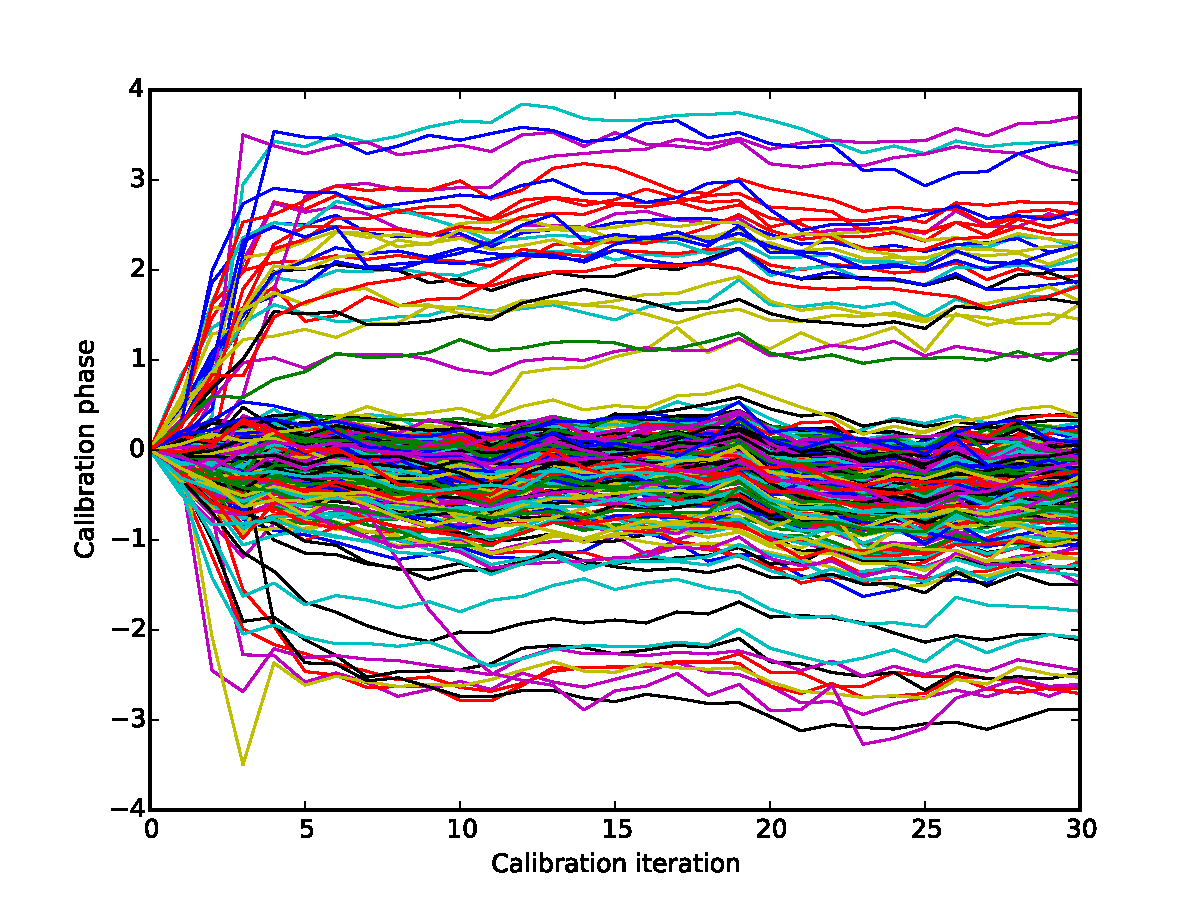
\includegraphics[width=\columnwidth]{figures/cal_paper_data_phases.pdf}
\caption{Gain phase solutions as a function of calibration iteration for an LWA TBN observation. The gain estimates are initialized with zero phase, but quickly span a $2\pi$ range, and settle into relatively flat, albeit noisy, solutions. The majority of phases congregate near zero, which is not surprising given the fairly good quality image produced from uncalibrated data.
}
\label{fig:data_phase}
\end{center}
\end{figure}

The gain amplitudes as a function of calibration iteration are shown in figure~\ref{fig:data_amp}. There is a fairly wide range in gain amplitudes (from 0.12 to 0.59). However, this is not surprising due to the non-uniformity in the cables from the antennas to the receivers. Again, the amplitudes are noisy by relatively flat.

\begin{figure}
\begin{center}
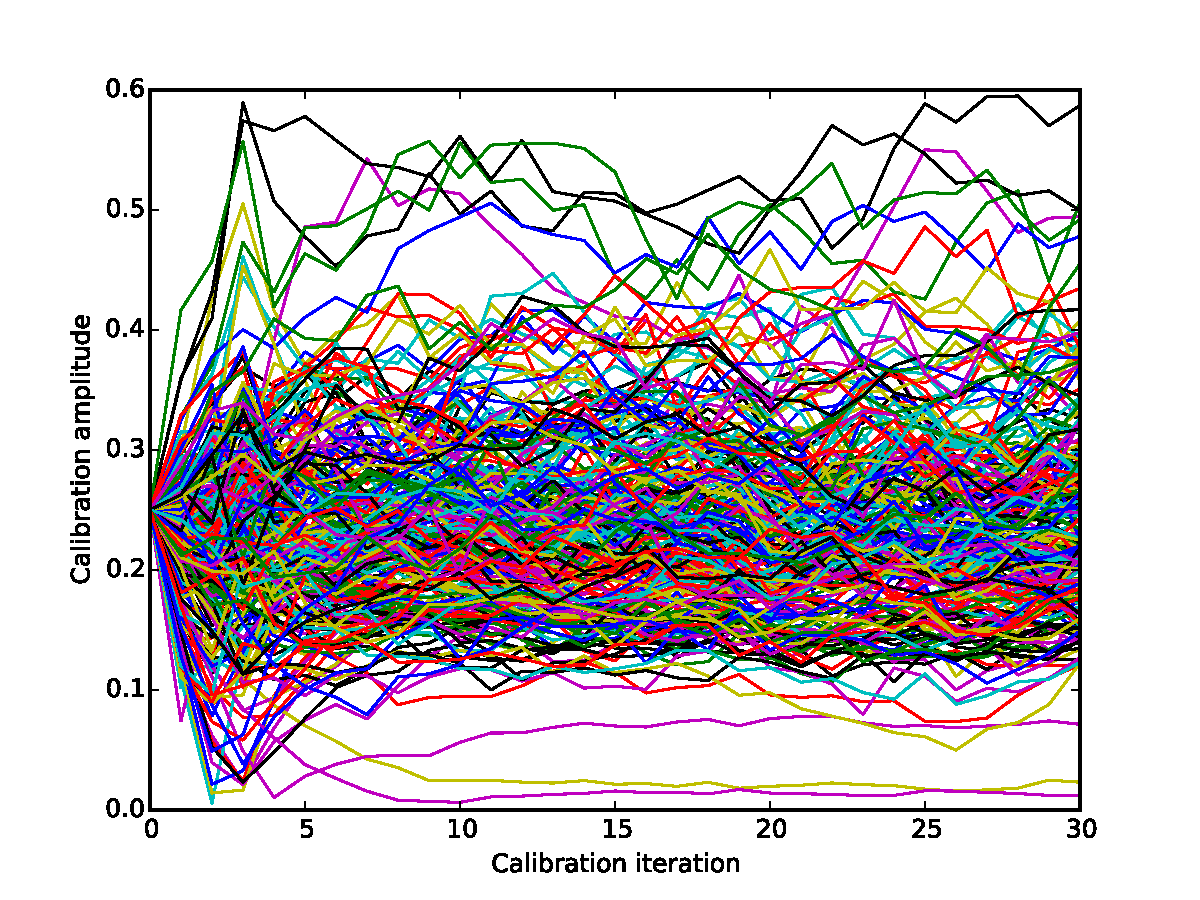
\includegraphics[width=\columnwidth]{figures/cal_paper_data_amps.pdf}
\caption{Gain amplitudes as a function of calibration iteration for an LWA TBN observation. The gains estimates were initialized with amplitude 0.25 after inspection of the electric field values compared to our model sky. The solutions are noisy, but flat. The range in amplitudes is due to the non-uniformity of cables between the LWA antennas and receivers.
}
\label{fig:data_amp}
\end{center}
\end{figure}

Figure~\ref{fig:data_images} shows the improvement in the images due to our calibration. The left panel shows the uncalibrated image integrated over 51.2 ms, 29 kHz. Cyg~A is prominent near the center of the image, and Cas~A is also clearly visible in the upper right. The middle panel shows the image produced after calibration with identical integration time and bandwidth. The sidelobes throughout the image are significantly suppressed, and the galactic plane is much more evident. We also note that the feature just to the right of Cyg~A is dimmer in the calibrated image, better matching the expected flux from the global sky model (GSM, \citealt{deo08}). We show the GSM modulated by two factors of the LWA primary beam in the right panel of figure~\ref{fig:data_images} for reference.

\begin{figure*}
\begin{center}
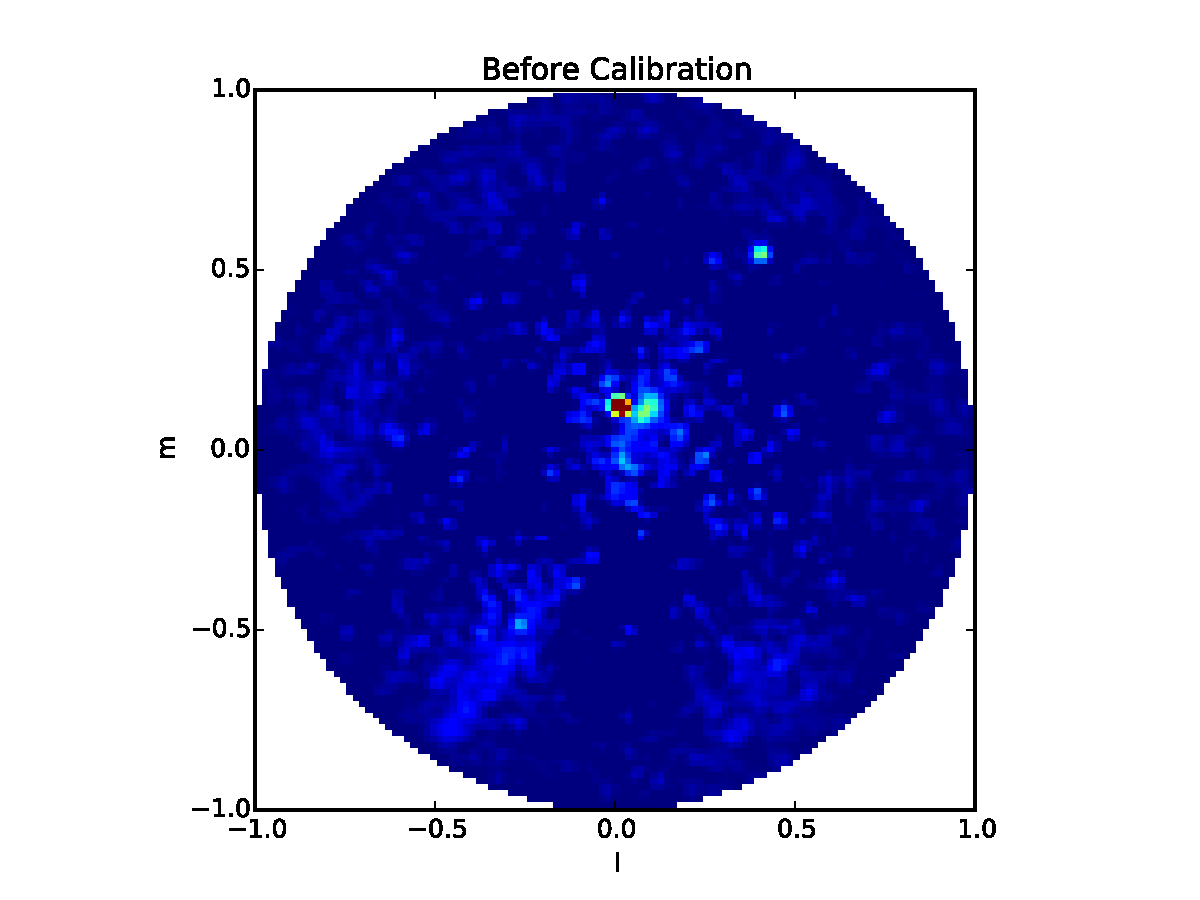
\includegraphics[width=0.33\linewidth]{figures/cal_paper_data_image_before.pdf}
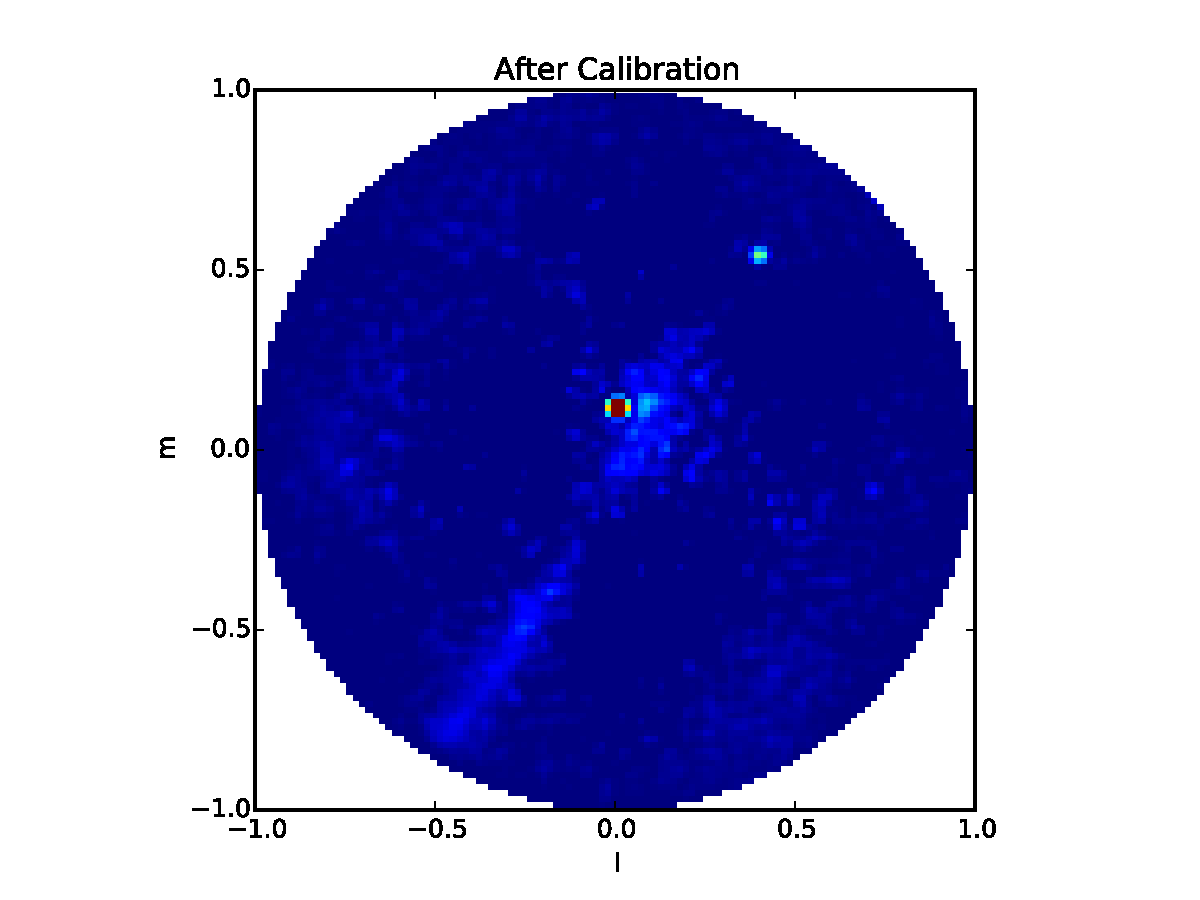
\includegraphics[width=0.33\linewidth]{figures/cal_paper_data_image_after.pdf}
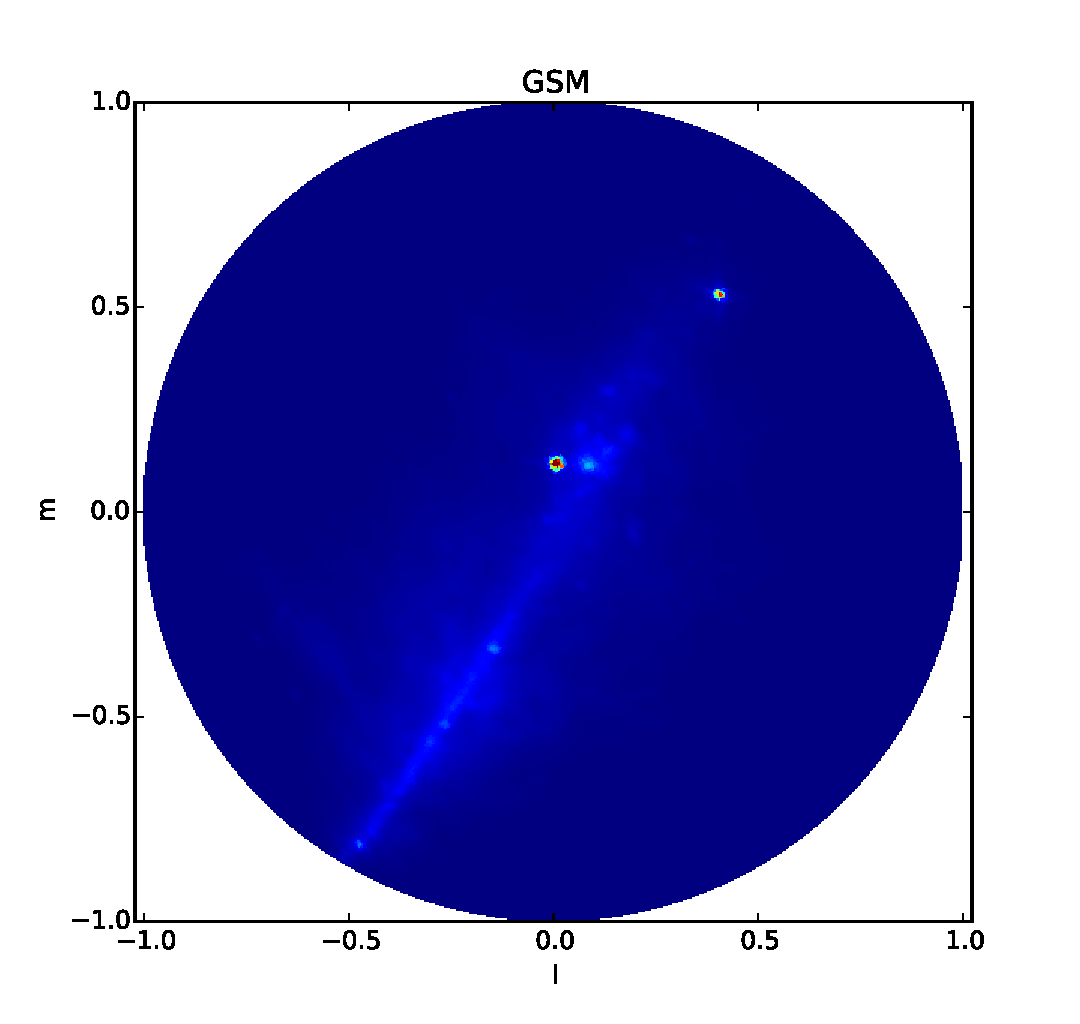
\includegraphics[width=0.33\linewidth]{figures/cal_paper_gsm_beam_weighted.pdf}
\caption{Images produced before (left) and after (middle) calibrating LWA data. These images were produces with 29 kHz bandwidth and 51.2 ms integration. The calibrated image shows significant reduction in sidelobe rumble throughout, while retaining the prominent Cyg~A and Cas~A sources. The galactic plane is also substantially more evident after calibration. For reference, the GSM is shown in the same coordinates and weighted by two factors of the LWA primary beam in the right panel.
}
\label{fig:data_images}
\end{center}
\end{figure*}

To compare the image qualities quantitatively we compute the dynamic range, defined as the peak of the image over the noise level. We estimate the noise level as the median of the absolute deviation of the image. With this metric we find the calibrated image to have a 55\% dynamic range improvement over the uncalibrated image.

\section{Noise analysis}\label{sec:noise}

Here we study the properties of our calibration solutions with respect to noise in the system. In order to compare to solutions from visibility-based calibration, we first derive the theoretical lower bound of the error in these solutions, given a set of measured visibilities, $\mathbf{V}$. We will do this through the Fischer information formalism and employ the Cram\'er-Rao lower bound 

Assume we did form visibilities with some integration time. Assuming the noise on each visibility, $\sigma_{ab}$, is independent, we can write the likelihood function of measuring $V_{ab}$ given the true value, the gains, and the noise.
\begin{equation}
\mathcal{L}(V_{ab};\mathbf{g}) = \frac{1}{2\pi \sigma_{ab}^2}\exp\left[-\frac{\left|V_{ab} - g_a g_b^* V_{ab}^T\right|^2}{2\sigma_{ab}^2}\right]
\end{equation}
Then the likelihood of the set of all visibilities is the product of all individual likelihoods.
\begin{equation}
\mathcal{L}(\mathbf{V};\mathbf{g}) = \prod_a \prod_{b > a} \mathcal{L}(V_{ab};\mathbf{g})
\end{equation}
The Fischer information matrix for the set of gain parameters is
\begin{equation}
\mathbf{F}^g_{ij} = \left<\left. \frac{\partial \ln \mathcal{L}(\mathbf{V};\mathbf{g})}{\partial g_i} \frac{\partial \ln \mathcal{L}(\mathbf{V};\mathbf{g})}{\partial g_j}\right|_\mathbf{g}\right>,
\end{equation}
where the expectation is taken over all possible visibility measurements.
We next evaluate the derivate of the log-likelihood.
\begin{equation}
\frac{\partial \ln \mathcal{L}(\mathbf{V};\mathbf{g})}{\partial g_i} = 
\sum_{a \ne i} \frac{g_a^* V_{ai}^{T*} (V_{ai} - g_a g_i^* V_{ai}^T)}{2 \sigma_{ai}^2}
\end{equation}

In order to find the Cram\'er-Rao lower bound on the variance of the complex parameter, $g_i$, we consider the term of the Fischer matrix where the first derivative is taken with respect to $g_i$, and the second with $g_i^*$. The result is
\begin{align}
\mathbf{F}^g_{ii} = & \left<\left[ \sum_{a \ne i} \frac{g_a^* V_{ai}^{T*} (V_{ai} - g_a g_i^* V_{ai}^T)}{2 \sigma_{ai}^2} \right] \right. \times \nonumber \\
& \left. \left[ \sum_{b \ne i} \frac{g_b V_{bi}^{T} (V_{bi}^* - g_b^* g_i V_{bi}^{T*})}{2 \sigma_{bi}^2} \right] \right> \nonumber \\
= &\sum_{a\ne i} \sum_{b \ne i} \frac{g_a^* g_b V_{ai}^{T*} V_{bi}^T}{4 \sigma_{ai}^2 \sigma_{bi}^2} \left< V_{ai}V_{bi}^* - g_i g_b^* V_{ai}V_{bi}^{T*}\nonumber \right.\\
&\left. - g_a g_i^* V_{ai}^T V_{bi}^* + g_a g_b^* |g_i|^2 V_{ai}^T V_{bi}^{T*}\right>
\label{eq:Fischer_before_expect}
\end{align}

The expected values are easy to evaluate. Each visibility will average to the ``true" value times the respective gains. The term with two visibilities will include a noise bias on autocorrelation terms.
\begin{equation}
\left<V_{ai}V_{bi}^*\right> = |g_i|^2 g_a g_b^* V_{ai}^T V_{bi}^{T*} + \sigma_{ai}^2 \delta_{ab}
\end{equation}
Here $\delta_{ab}$ is the Kronecker delta selecting the term where $a=b$ and the noise correlates. Plugging in the expectation values, equation \ref{eq:Fischer_before_expect} simplifies greatly to
\begin{equation}
\mathbf{F}^g_{ii} = \sum_{a \ne i} \frac{\left|g_a V_{ia}^T \right|^2}{4\sigma_{ai}^2}
\end{equation}

Finally we relate our result to the theoretical best uncertainty we can place on our unknown gain parameter using the Cram\'er-Rao lower bound.
\begin{equation}\label{eq:cramer_rao}
\sigma_{g_i}^2 \ge \left[ \mathbf{F}^g_{ii} \right]^{-1} = \left[ \sum_{a \ne i} \frac{\left|g_a V_{ia}^T \right|^2}{4\sigma_{ai}^2} \right]^{-1}
\end{equation}

We next run a set of EPICal simulations to compare the noisy results to the theoretical lower bound given a set of equivalent visibilities. Each simulation is run with a simple sky of a single point source with flux 1 Jy. We add noise to the system by adding a Gaussian-random complex value to each channelized electric field antenna measurement as in equation~\ref{eq:apply_gain}. The ``true" gains in our simulation are unity, as well as our initial estimate. This emulates a system where the initially volatile gain correction has been suppressed and only noise remains to corrupt our estimation, allowing us to run many simulations on a shorter timescale.

We vary two parameters in our simulations: the amount of noise added to our measurements, and the length of integration in each calibration loop. 

\section{Discussion}\label{sec:discussion}

\section*{Acknowledgements}
This work has been supported by the National Science Foundation through award AST-1206552.


%%%%%%%%%%%%%%%%%%%% REFERENCES %%%%%%%%%%%%%%%%%%

% The best way to enter references is to use BibTeX:

\bibliographystyle{../mnras}
\bibliography{../epic} % if your bibtex file is called example.bib



%%%%%%%%%%%%%%%%% APPENDICES %%%%%%%%%%%%%%%%%%%%%

%\appendix

%\section{Some extra material}

%If you want to present additional material which would interrupt the flow of the main paper,
%it can be placed in an Appendix which appears after the list of references.

%%%%%%%%%%%%%%%%%%%%%%%%%%%%%%%%%%%%%%%%%%%%%%%%%%


% Don't change these lines
\bsp	% typesetting comment
\label{lastpage}
\end{document}

% End of mnras_template.tex

% Don't change these lines
\bsp	% typesetting comment
\label{lastpage}
\end{document}

% End of mnras_template.tex